
\documentclass[a4paper,11pt]{book}

% PAQUETES
\usepackage{./estilo/paquetes}
\usepackage{./estilo/colores}
\usepackage{./estilo/comandos}
\usepackage{colortbl}
\usepackage[utf8]{inputenc}

\graphicspath{{./img/}} 

\title{Manual de usuario}
\author{José Ángel Parada Jiménez}

\begin{document}

\section{Introduction}
This section describes the most significant for understanding the operation of the system. Any questions you have the application user on the operation of the same will solve making use of this manual or by contacting the developer of the application.

\section{Utilization}

\subsection {Login screen}
To use all the features of the system, the user of the application must loguarse it through the login screen:

\begin{figure}[!htb]
  \centering
    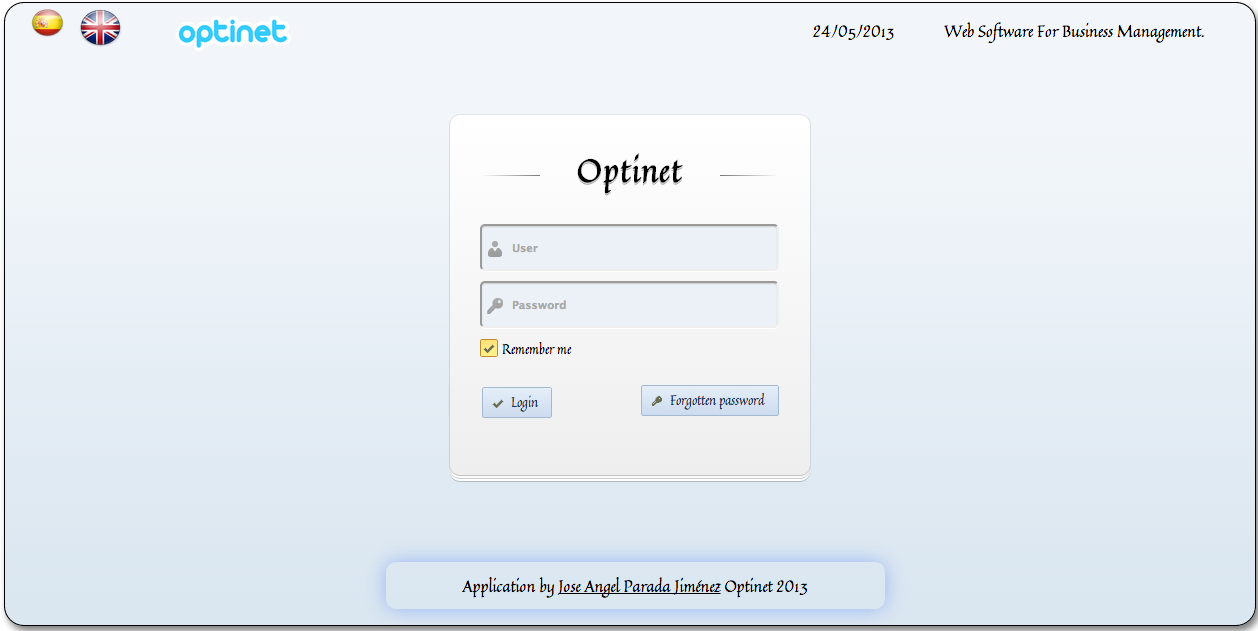
\includegraphics[scale=0.35]{icaplogin.png}
  \caption{Login screen}
  \label{a}
\end{figure}

In this screen it you can see how it will look in the other application screens. Any error in the login form appear below the buttons. The user is given the ability to remember the password, if this option is checked it will remember your password for 30 minutes. The user can send an email to the developer of the application by clicking on its name to be underlined. At the top, which is visible to other screens, you can see the connected user, the role you have and the current date. The user can change the language in any application screen, including this one from logging. Depending on the user's role to connect the system displays only the actions that user can perform:
\begin{itemize}
\item Administrator: is displayed in a dropdown up menu named Admin.
\item Doctor: You have an option to create report in the reports menu.
\end{itemize}

\newpage
\subsection {Forgot Password Screen}

\begin{figure}[!htb]
  \centering
    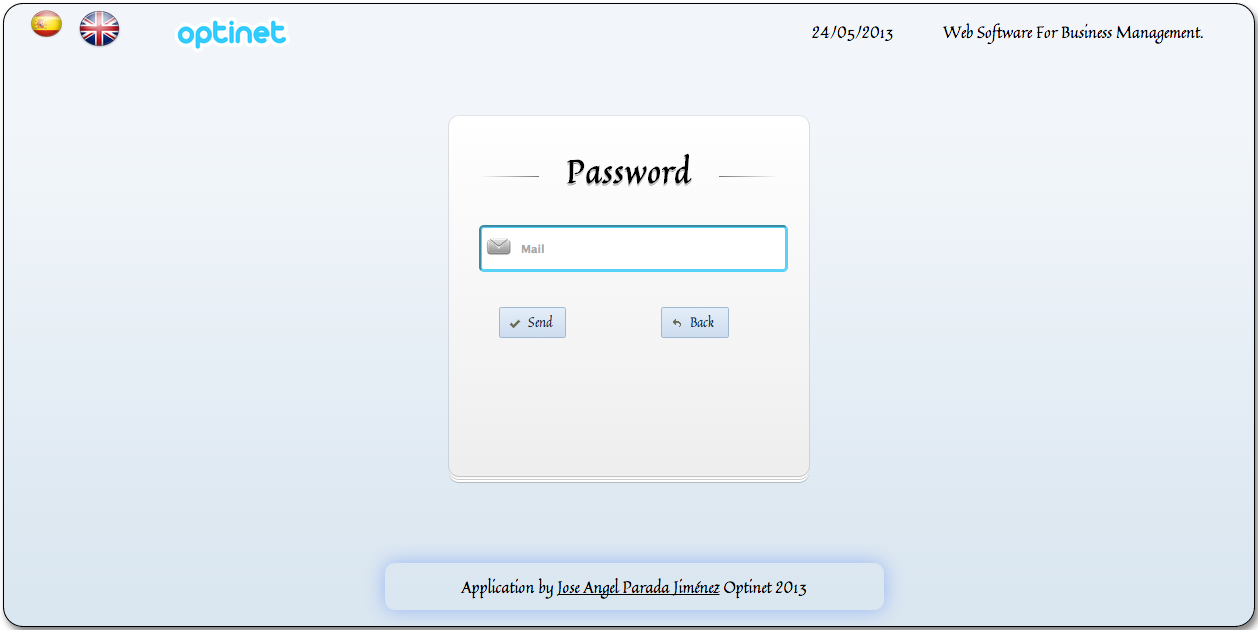
\includegraphics[scale=0.35]{icapolvidada.png}
  \caption{Forgot Password Screen}
  \label{a}
\end{figure}

In this screen any user of the application can recover your forgotten password email indicating your. The system will send you an email with a link reestablishment email the password to which only valid for single use only, if you click on this link will generate a new password for the user and we will send a new password to your email. Below the buttons you would see if you have sent the email or else an error occurred.

\newpage
\subsection {Main screen}

\begin{figure}[!htb]
  \centering
    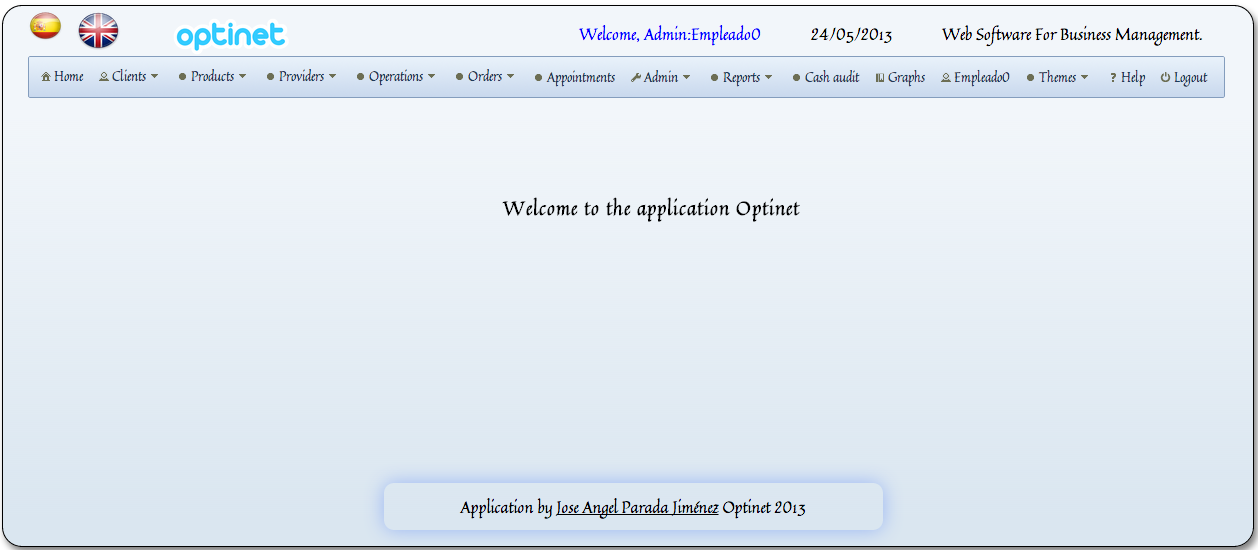
\includegraphics[scale=0.35]{icapprincipal.png}
  \caption{Main screen}
  \label{a}
\end{figure}

This is the screen that the application user sees when logging on to the system. Here the user can now use all the functionality of the system including language change or change the visual theme.

\subsection {Customer registration screen}

\begin{figure}[!htb]
  \centering
    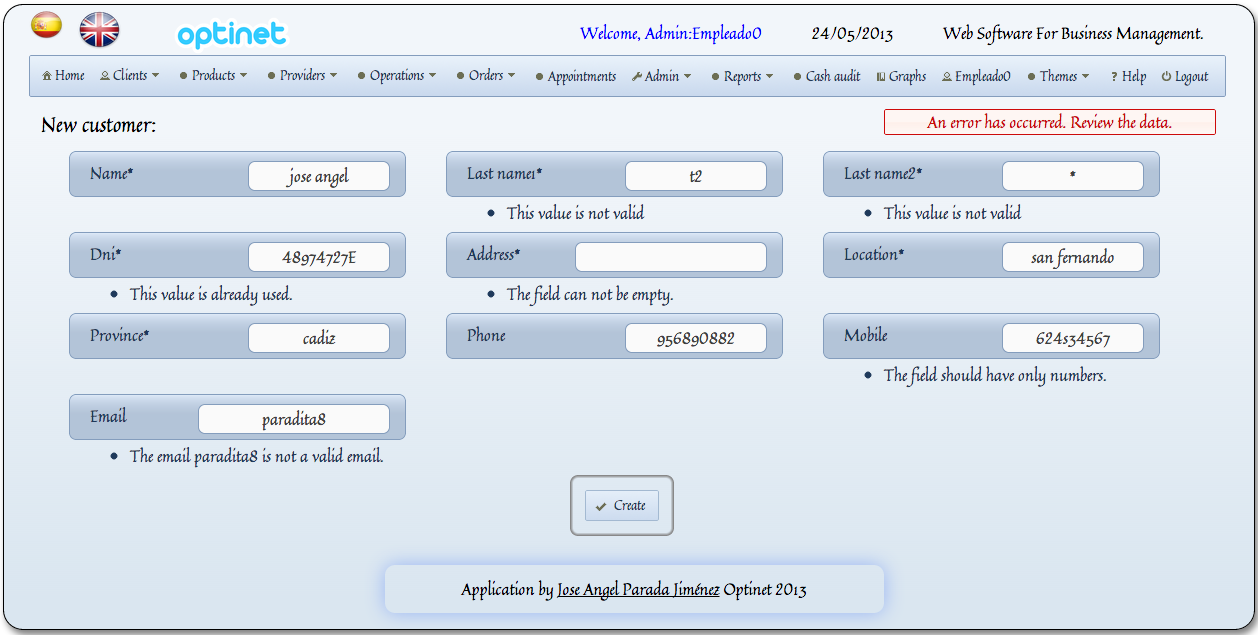
\includegraphics[scale=0.35]{icapregistrocliente.png}
  \caption{Customer registration screen}
  \label{a}
\end{figure}

In this screen the user of the application can register a new customer in the system. If any type of error in data entry will display an error message at the top right of the screen and the errors will be reflected under each input field.

\subsection {Screen clients list}

\begin{figure}[!htb]
  \centering
    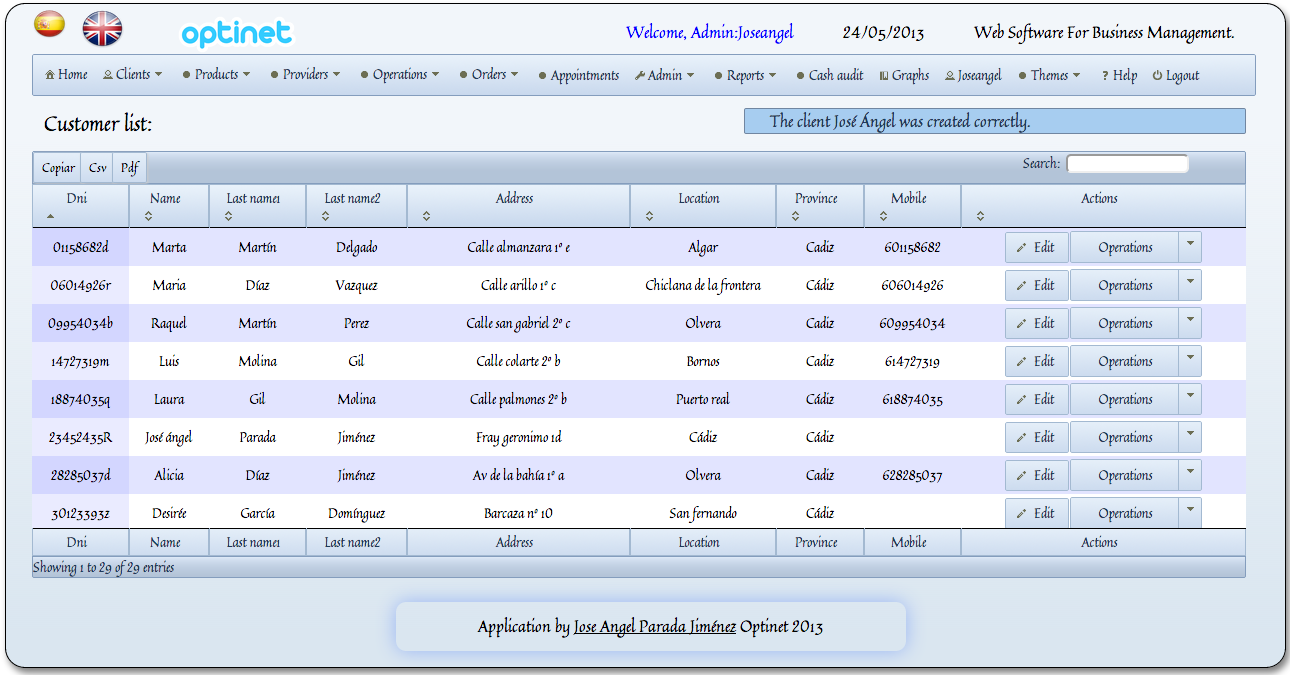
\includegraphics[scale=0.35]{icaplistarclientes.png}
  \caption{Screen clients list}
  \label{a}
\end{figure}

In this screen the user of the client application can query stored in the system. The table gives the user the option to sort any column or search the field at the top right of the table. It also offers the ability to copy to the clipboard, copy in CSV format or a PDF of the data shown in the table. The user can perform any customer choice by clicking the drop-down operations. When you create, modify, or delete a client from the system will redirect the user to the application to this page where you can see the message of successful operation in the top right.

\newpage
\subsection {Display modify customer}

\begin{figure}[!htb]
  \centering
    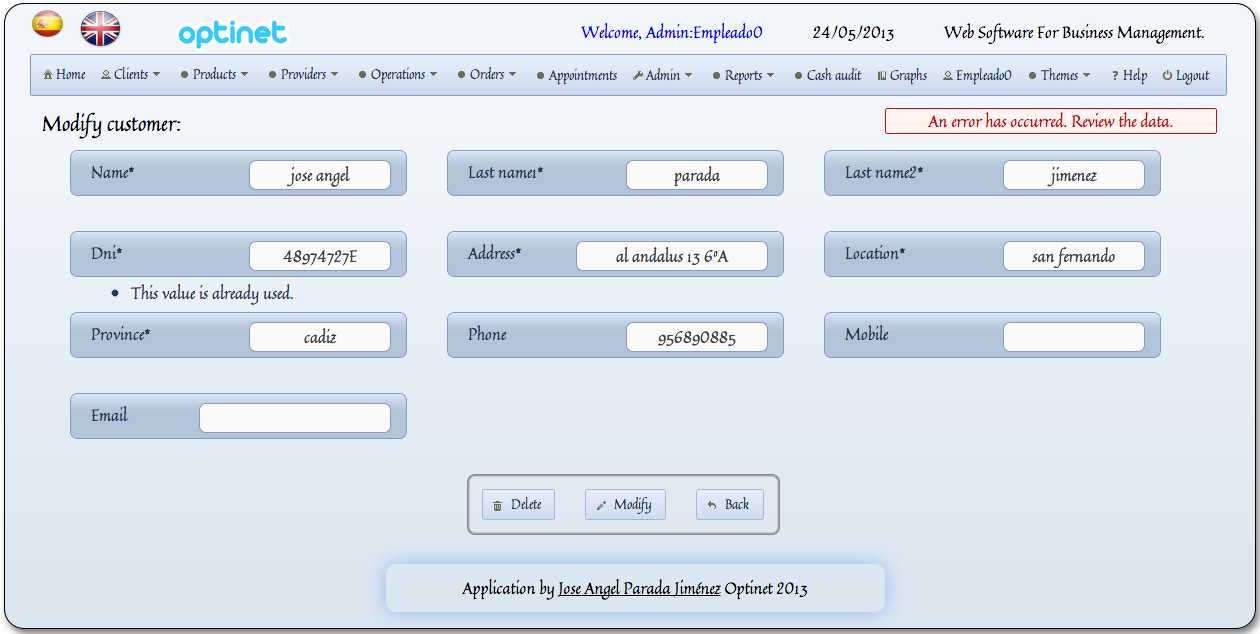
\includegraphics[scale=0.35]{icapmodificarcliente.png}
  \caption{Display modify customer}
  \label{a}
\end{figure}

In this screen the user can modify the application to a customer in the system. If any type of error in data entry will display an error message at the top right of the screen and the errors will be reflected under each input field. In this screen also offers the possibility of eliminating a system client, taking into account which can only be removed if no associated operations, otherwise disabled button is displayed and a message is displayed by placing the cursor over the button disabled.

\newpage
\subsection {Screen move products}

\begin{figure}[!htb]
  \centering
    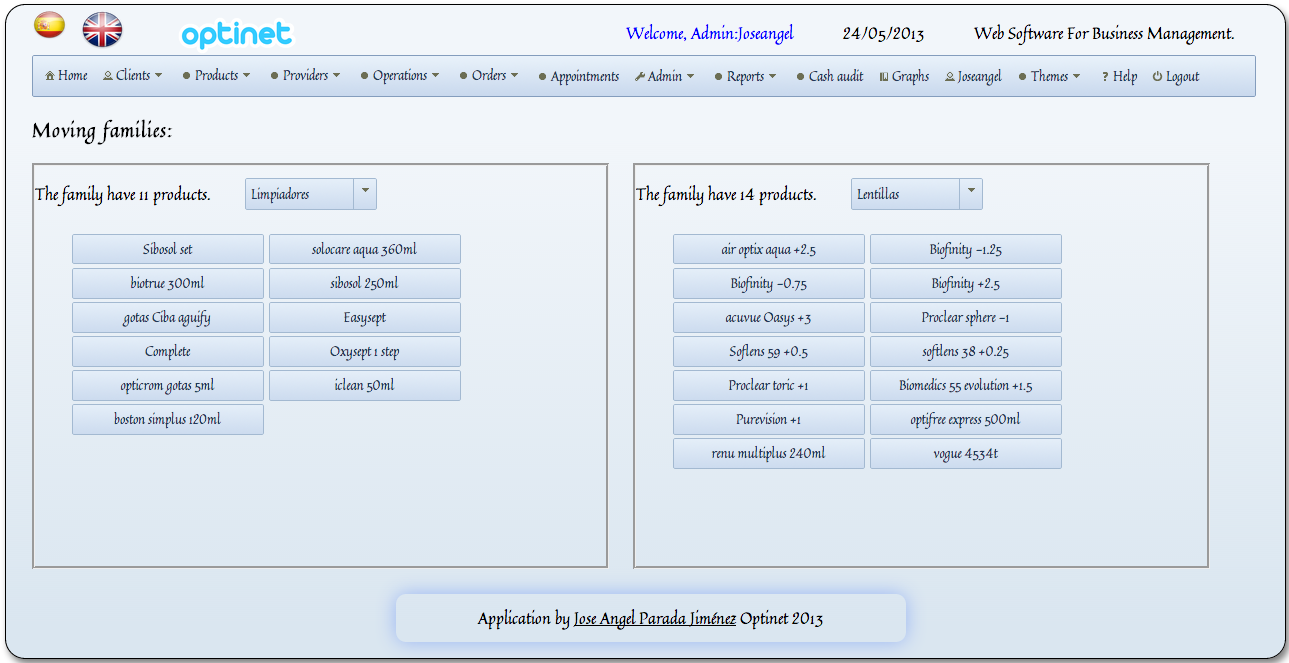
\includegraphics[scale=0.35]{icapmoverproductos.png}
  \caption{Screen move products}
  \label{a}
\end{figure}

In this screen the user of the application can move products between family system. The user can drag the items to the family you want or leave them in the family and also down the option for family products.

\subsection {Product registration screen}

\begin{figure}[!htb]
  \centering
    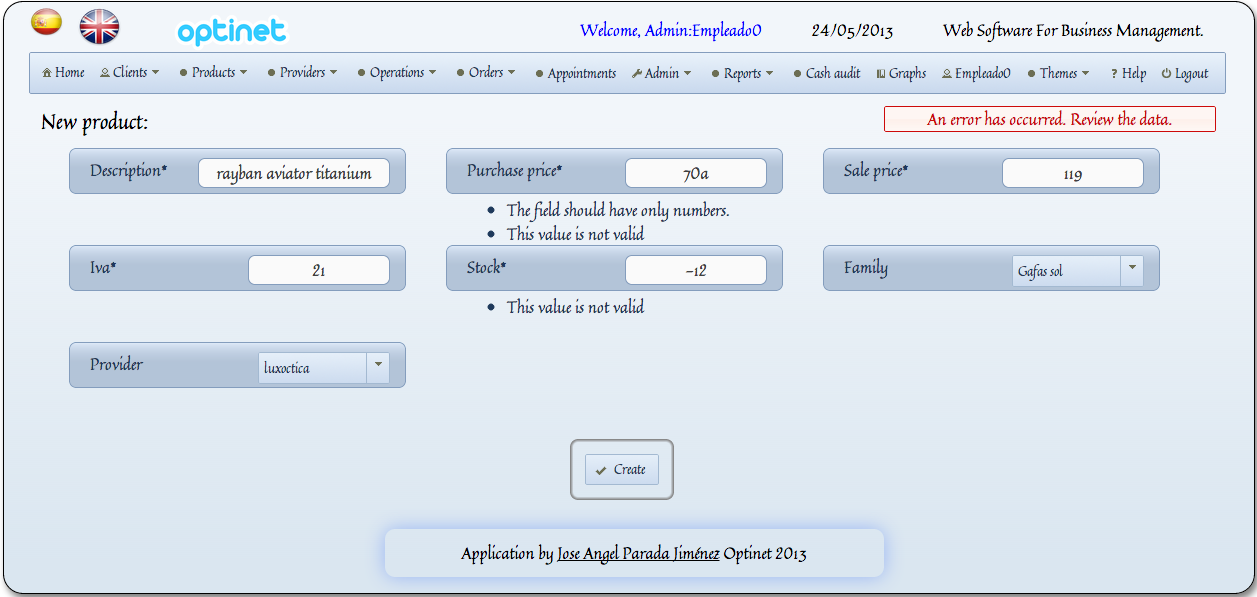
\includegraphics[scale=0.35]{icapregistroproducto.png}
  \caption{Product registration screen}
  \label{a}
\end{figure}

In this screen the user of the application can register a product in the system. If any type of error in data entry will display an error message at the top right of the screen and the errors will be reflected under each input field. The user can insert a new product without indicating the family to which it belongs or the vendor supplying that product.


\subsection {Display product change}

\begin{figure}[!htb]
  \centering
    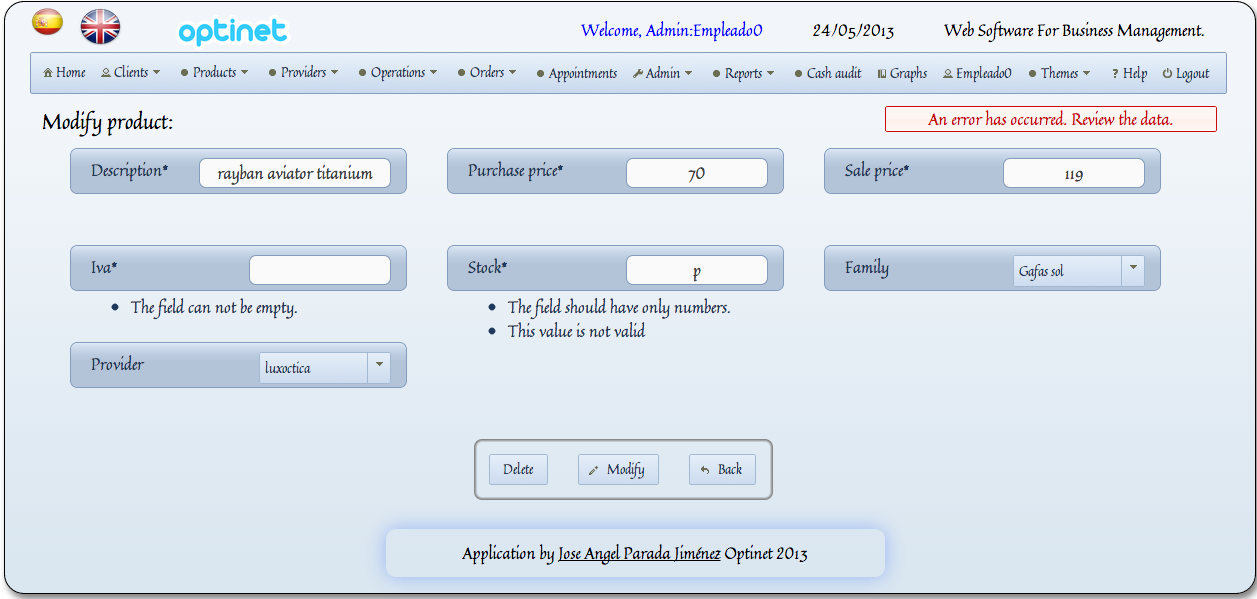
\includegraphics[scale=0.35]{icapmodificarproducto.png}
  \caption{Display product change}
  \label{a}
\end{figure}

In this screen the user can modify the application to a product in the system. If any type of error in data entry will display an error message at the top right of the screen and the errors will be reflected under each input field. In this screen also offers the possibility of eliminating a product of the system, taking into account which can only be removed if no associated operations, otherwise disabled button is displayed and a message is displayed by placing the cursor over the button disabled .
\newpage
\subsection {Display list products}

\begin{figure}[!htb]
  \centering
    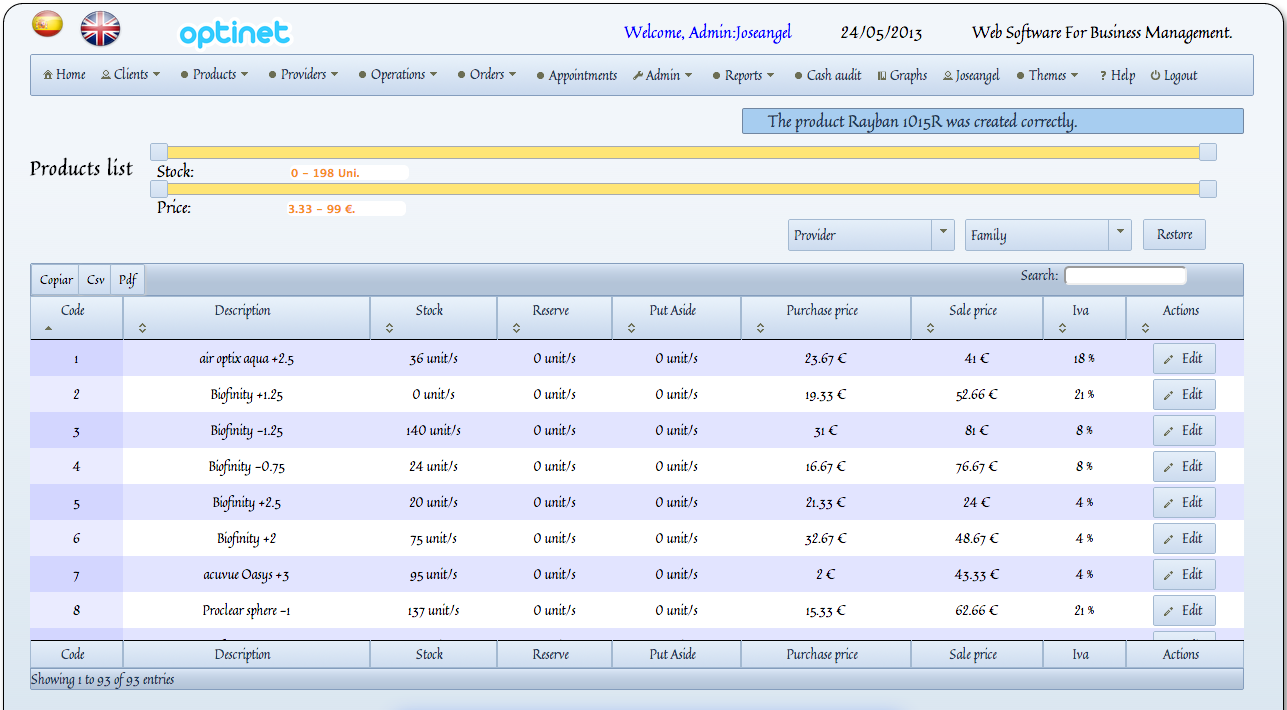
\includegraphics[scale=0.35]{icaplistarproductos.png}
  \caption{Display list products}
  \label{a}
\end{figure}

In this screen the user of the application can query the products stored in the system. The table gives the user the option to sort any column or search the field at the top right of the table. It also offers the ability to copy to the clipboard, copy in csv format or a PDF of the data shown in the table. At the top the user can perform filtered down changing table or sliders. When you create, modify, or delete a product of the system will redirect the user to the application to this page where you can see the message of successful operation in the top right.


\newpage
\subsection {Screen families list}

\begin{figure}[!htb]
  \centering
    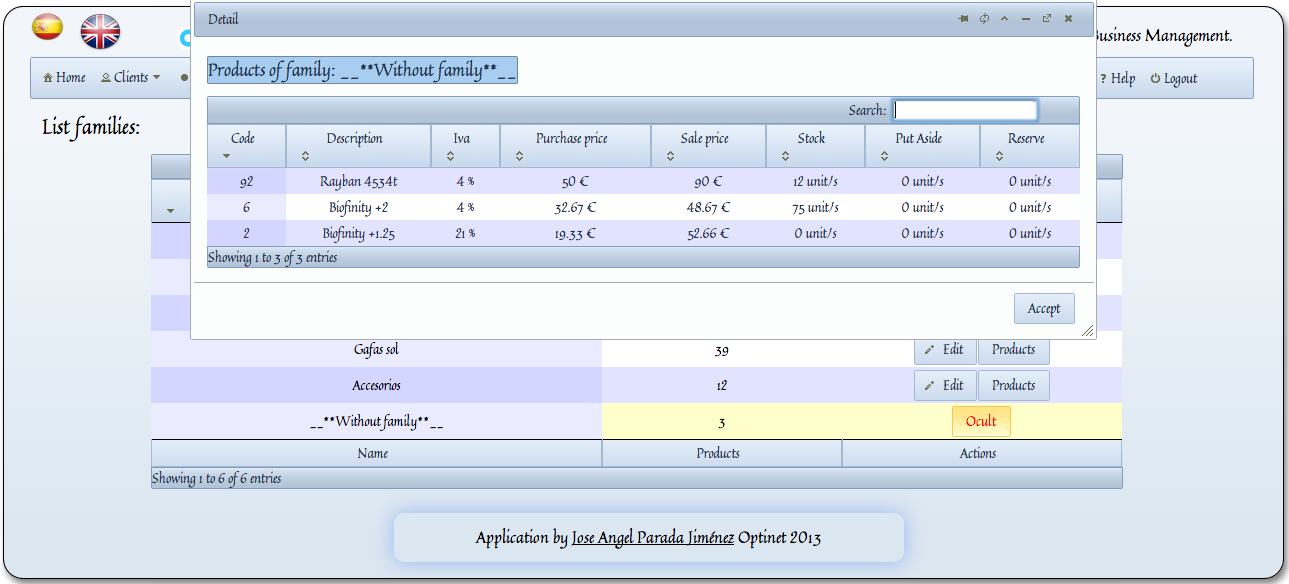
\includegraphics[scale=0.35]{icaplistarfamilias.png}
  \caption{Screen families list}
  \label{a}
\end{figure}

In this screen the user of the application can query the families stored in the system. It offers the user the opportunity to view the products in a given family by clicking the Products button. This option is also available in the display list providers to consult the products supplied by a particular supplier.

\newpage
\subsection {Display new sale}

\begin{figure}[!htb]
  \centering
    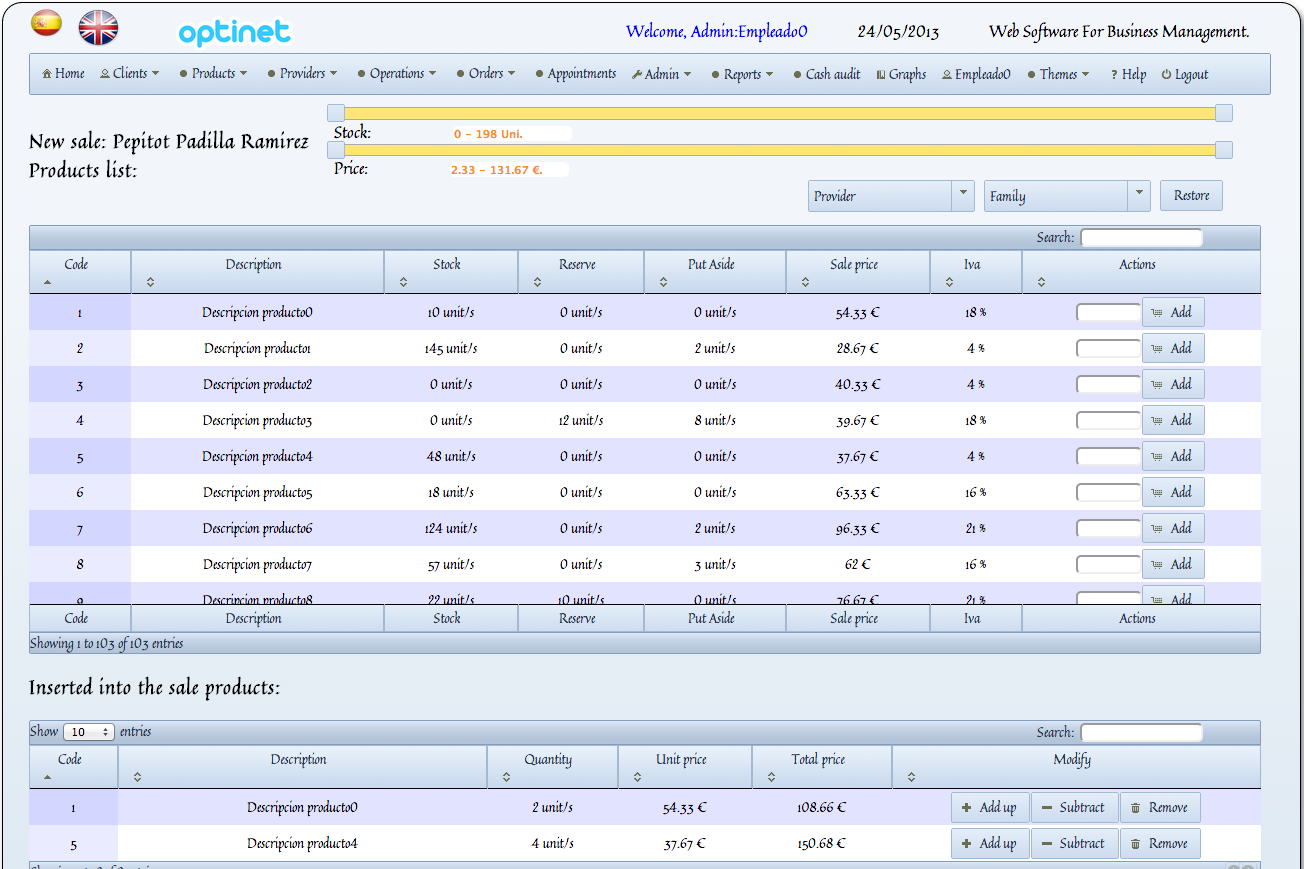
\includegraphics[scale=0.35]{icapnuevaventa.png}
  \caption{Display new sale}
  \label{a}
\end{figure}

\begin{figure}[!htb]
  \centering
    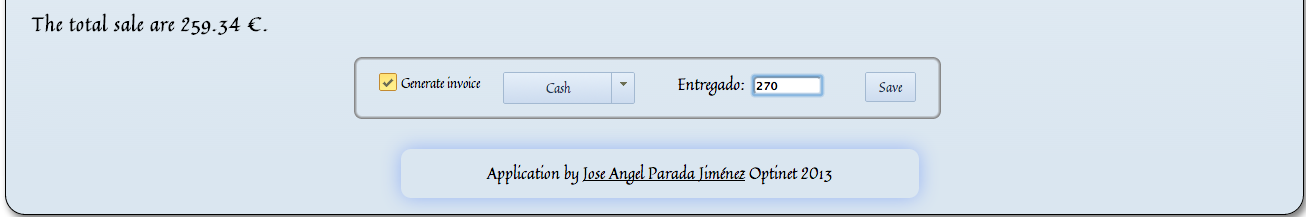
\includegraphics[scale=0.35]{icapnuevaventa1.png}
  \caption{Display new sale 1}
  \label{a}
\end{figure}

\begin{figure}[!htb]
  \centering
    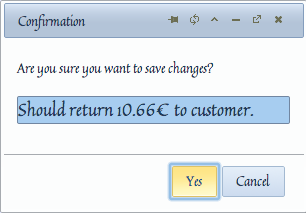
\includegraphics[scale=0.35]{icapnuevaventa2.png}
  \caption{Display new sale 2}
  \label{a}
\end{figure}

In this screen the user of the application can create a new sell in the system. First you will see a table where the user will choose the client that wants to make a sale. At the top the user can perform filtered down changing table or sliders. As indicated from unveil products in the table below and can increase, decrease or eliminate any of these products from the same table. Any data entered incorrectly displays an error message. The user can choose to display at that moment the sales document or customer payment, cash or card. If the card was delivered text field disappear. Clicking the save button will display a message confirming the sale, it will include the amount to be returned to the customer if cash was chosen, otherwise just show the confirmation message. Once the sale has been made just redirect the user to the sales list.

\subsection {Display sales list}

\begin{figure}[!htb]
  \centering
    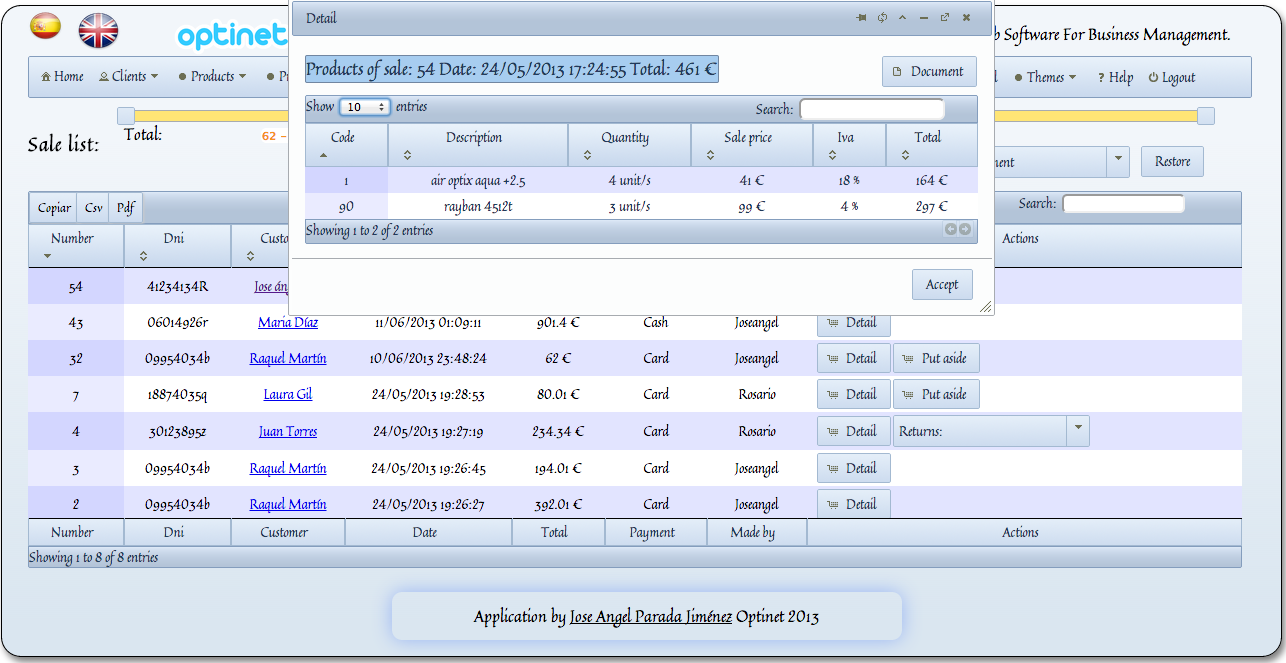
\includegraphics[scale=0.35]{icaplistarventas.png}
  \caption{Display sales list}
  \label{a}
\end{figure}

In this screen the user can see the sales application created in the system. It gives the user the possibility to filtered down the table and the top sliders, including filter also make a range of dates. The user can view the details of a particular sale, showing the associated products, the sales document and may also, clicking on the name of the client, see client data. You can also show if there is, the return of a sale by clicking on the drop down returns.

\newpage
\subsection {Screen new return}

\begin{figure}[!htb]
  \centering
    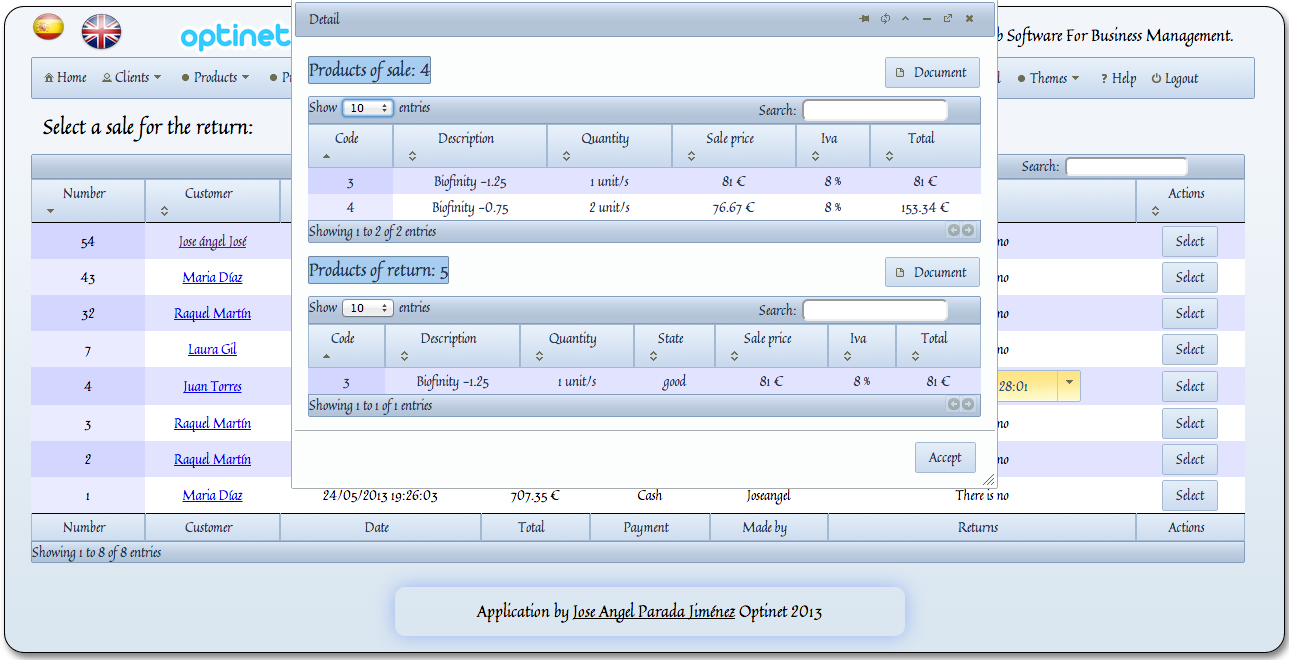
\includegraphics[scale=0.35]{icapnuevadevolucion.png}
  \caption{Screen new return}
  \label{a}
\end{figure}


\begin{figure}[!htb]
  \centering
    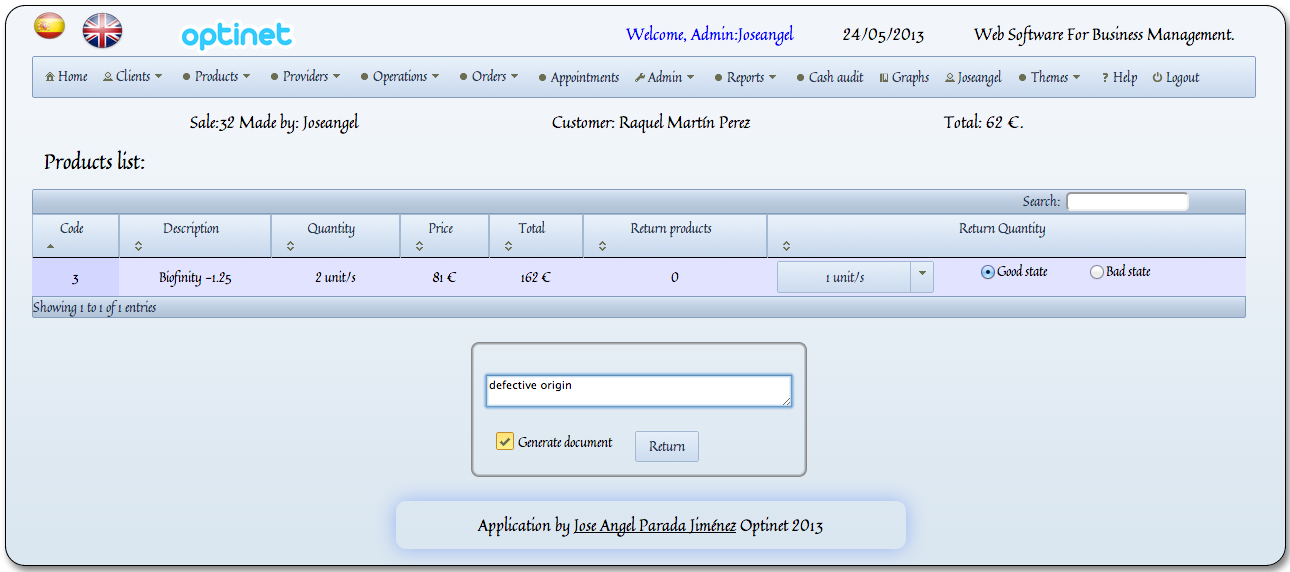
\includegraphics[scale=0.35]{icapnuevadevolucion1.png}
  \caption{Screen new return 1}
  \label{a}
\end{figure}

In this screen the user can create a new application in the system return. First you will see a table where the user will choose the sale to which you want to make the return. The user will select the quantities of the products of that sale you want to return and status. If the condition is good, it would increase the stocks. The way back to the customer will be the same with which the sale was made. The user can choose to display at that moment the return document. Clicking the save button will display a message to confirm the return. Once the return has been made just redirect the user to the list of returns.

\newpage
\subsection {Display list reservations}

\begin{figure}[!htb]
  \centering
    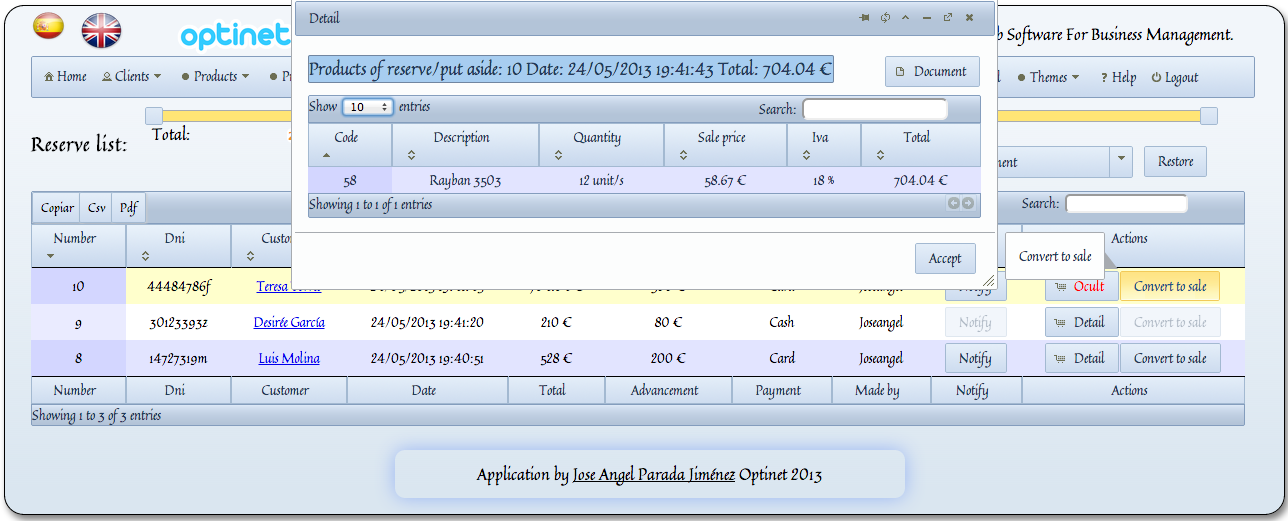
\includegraphics[scale=0.35]{icaplistarreservas.png}
  \caption{Display list reservations}
  \label{a}
\end{figure}

In this screen the user of the application can see the reserves created in the system. It gives the user the possibility to filtered down the table and the top sliders, including filter also make a range of dates. The user can view the details of a particular reservation, showing the associated products, the document can also backup and clicking on the name of the client, see client data. The user can make a reservation sale if the products are already available or register the notice to the customer to come and collect the reservation. If it can not tell the customer that the products are not available or have been converted already on sale, the button will alert desactivado.Si could not make sales because the products are not available also button appears disabled.

\newpage
\subsection {Display list operations}

\begin{figure}[!htb]
  \centering
    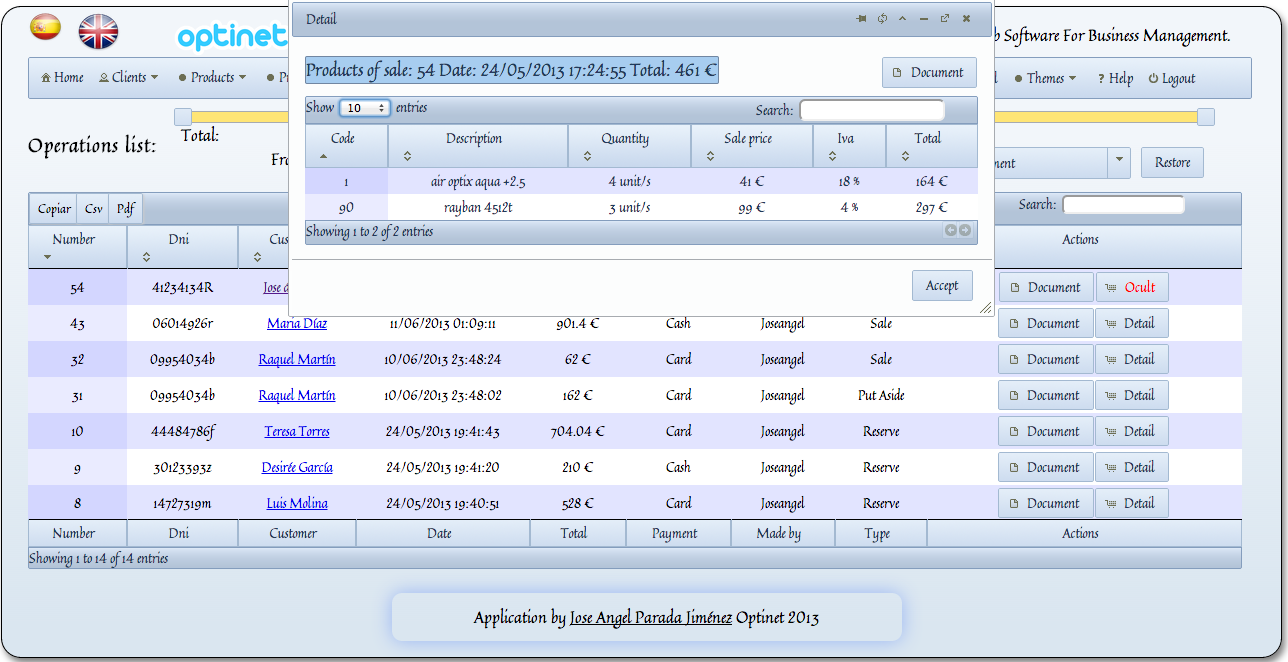
\includegraphics[scale=0.35]{icaplistaroperaciones.png}
  \caption{Display list operations}
  \label{a}
\end{figure}

In this screen the user of the application can see all the transactions created in the system (sales, returns, reserves, section). It gives the user, as always, the possibility to perform the filtrates that are needed to search and also indicate that on this screen, for example, you could see the operations that a particular customer has made . The user can view the document associated with the type of operation by clicking on document, or you could see the products associated with a particular operation by pressing the button detail.

\newpage
\subsection {Display new order}

\begin{figure}[!htb]
  \centering
    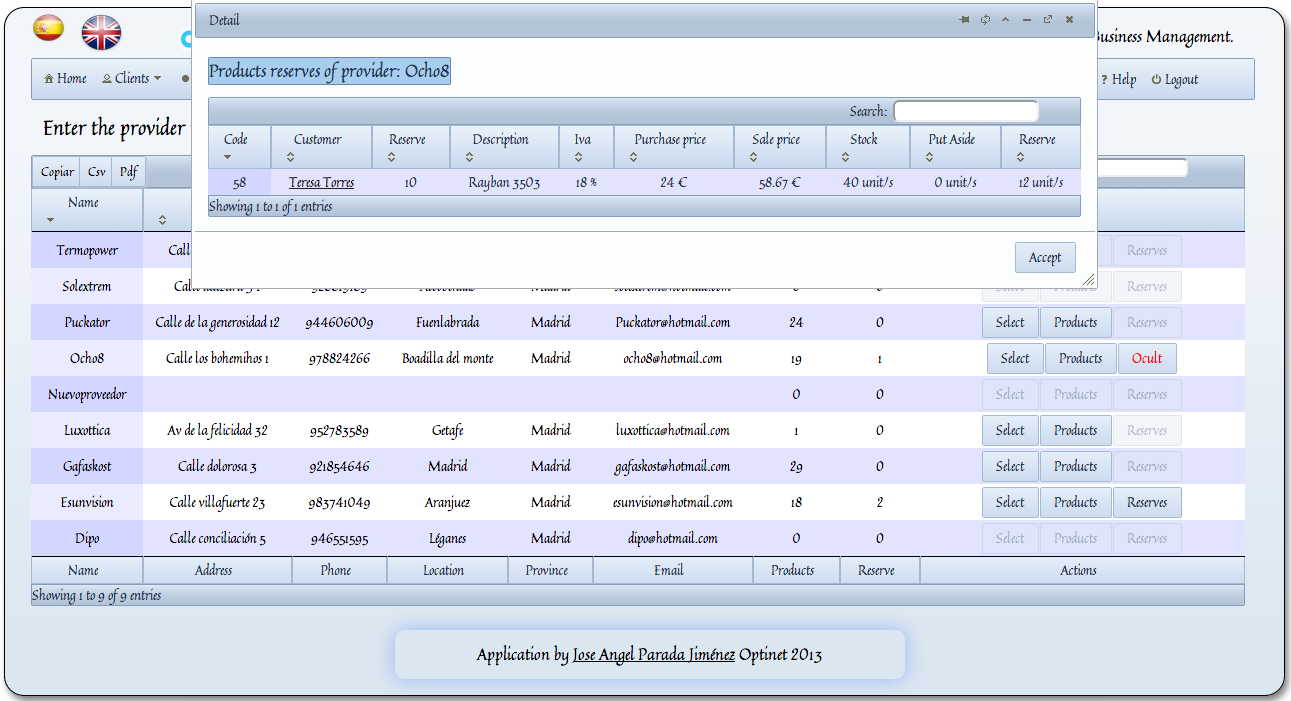
\includegraphics[scale=0.35]{icapnuevopedido.png}
  \caption{Display new order}
  \label{a}
\end{figure}

In this screen the user of the application can create a new order from a particular supplier. First the user will be shown a screen where you can see some product providers who have booked, consult each vendor supplied products or see in that book are reserved products. The user must select the provider you want to make an order.

\newpage
\begin{figure}[!htb]
  \centering
    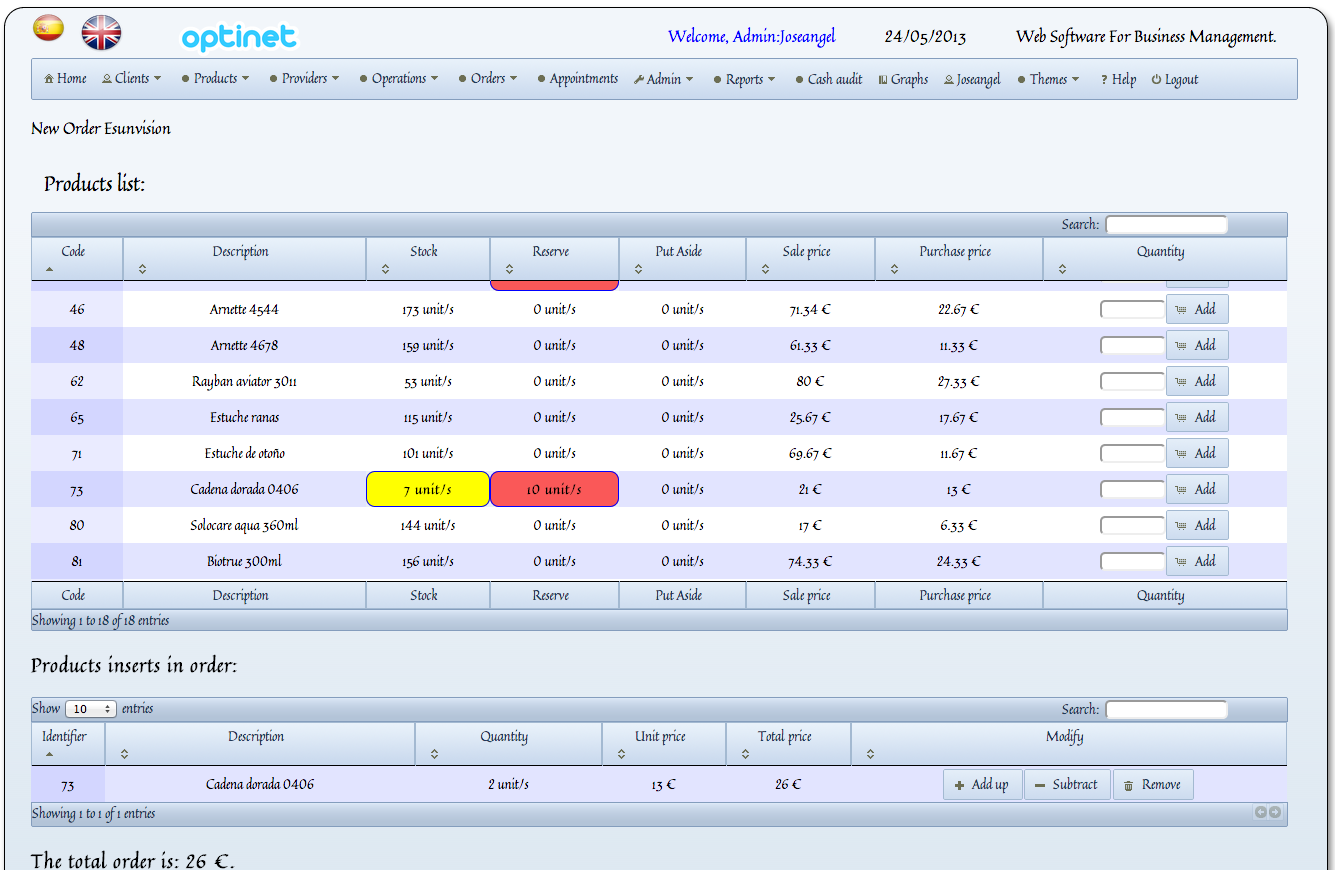
\includegraphics[scale=0.35]{icapnuevopedido1.png}
  \caption{Display new order 1}
  \label{a}
\end{figure}

On this screen you will enter the products you want to perform to the supplier. Are displayed in a yellow box products with less than 10 stocks with a red box items reserved for the user to see clearly the needs of the system.

\subsection {Display Order list}

\begin{figure}[!htb]
  \centering
    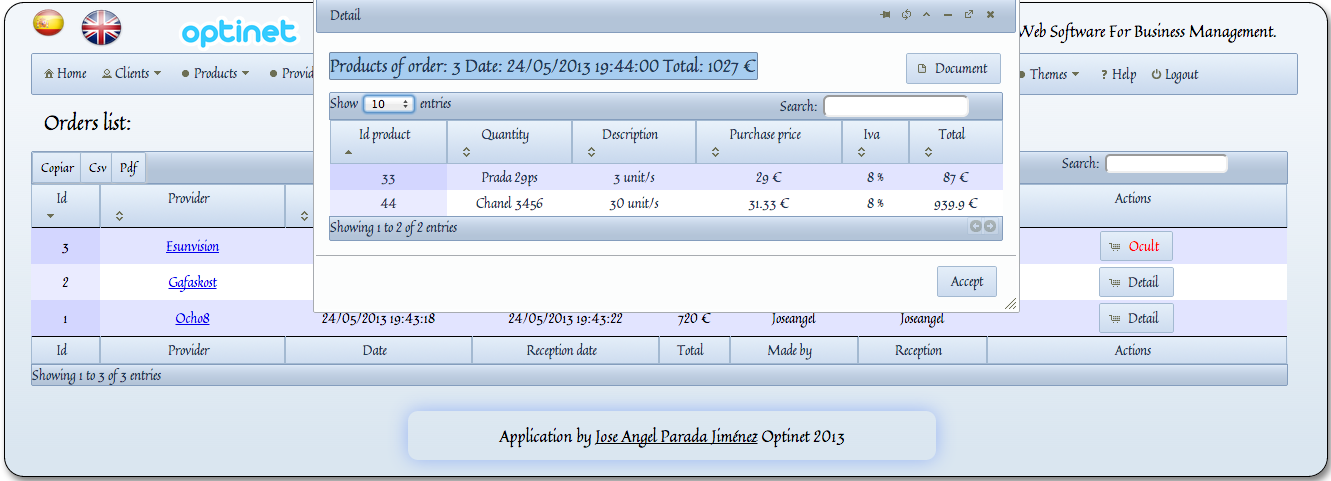
\includegraphics[scale=0.35]{icaplistarpedidos.png}
  \caption{Display Order list}
  \label{a}
\end{figure}

In this screen the user of the application can view all orders. This is where the user can recepcionar orders placed stored the user who recepcionado, updated date and product stocks. You will also see related products show an order or other ordering document.

\subsection {Display dating}

\begin{figure}[!htb]
  \centering
    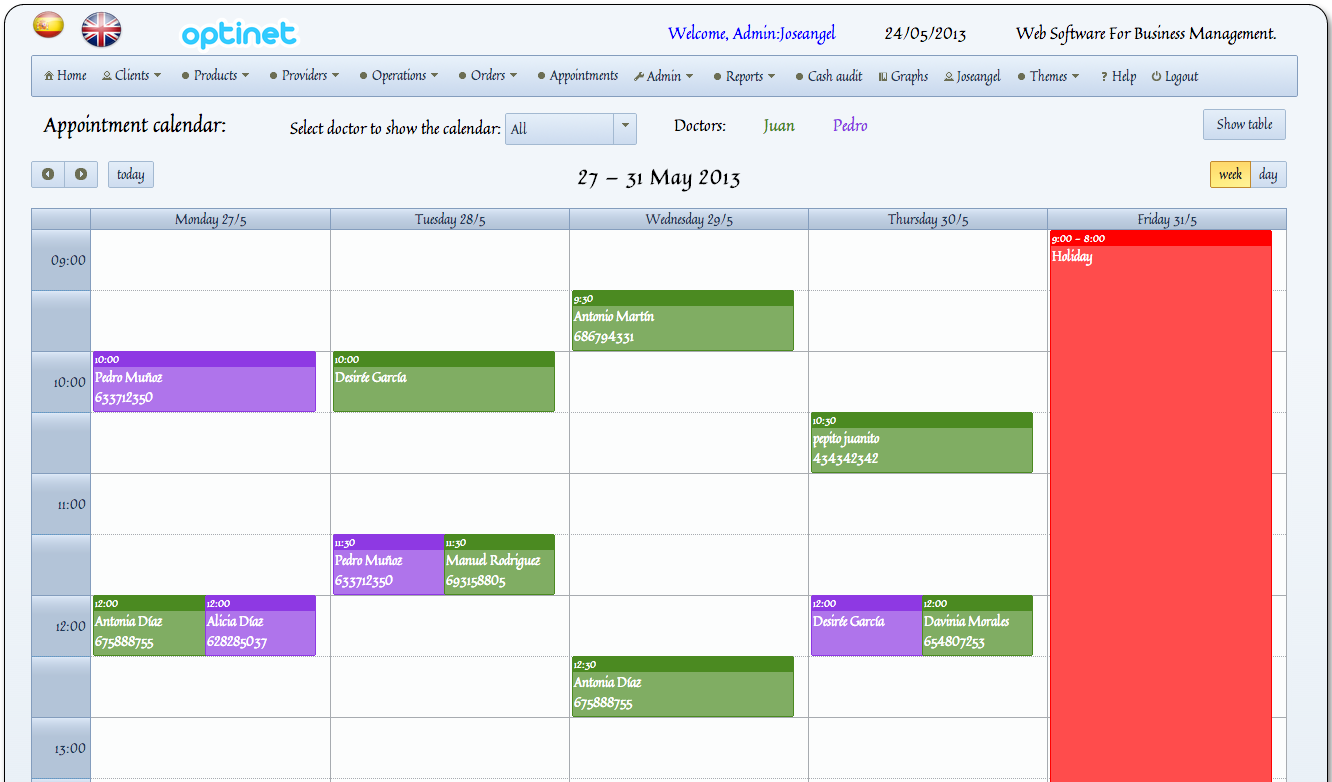
\includegraphics[scale=0.35]{icapcitas.png}
  \caption{Display dating}
  \label{a}
\end{figure}

In this screen the user can manage appointments either create a new appointment or delete an appointment. The user has the ability to display in the calendar only a certain doctor appointments. To delete an appointment will be pressed in the event and displays a message asking if you really want to delete the appointment system. To perform citation searches faster or print a document dating, you can press the button show table on the top right of the screen. The system will not be stored dating days prior to the current date. The colors of the quotes belong to the color associated with the doctor that the administrator can change the modification of employee screen. If holiday pulsase above, the system would not create an appointment and you can not create appointments on a holiday.

\newpage
\begin{figure}[!htb]
  \centering
    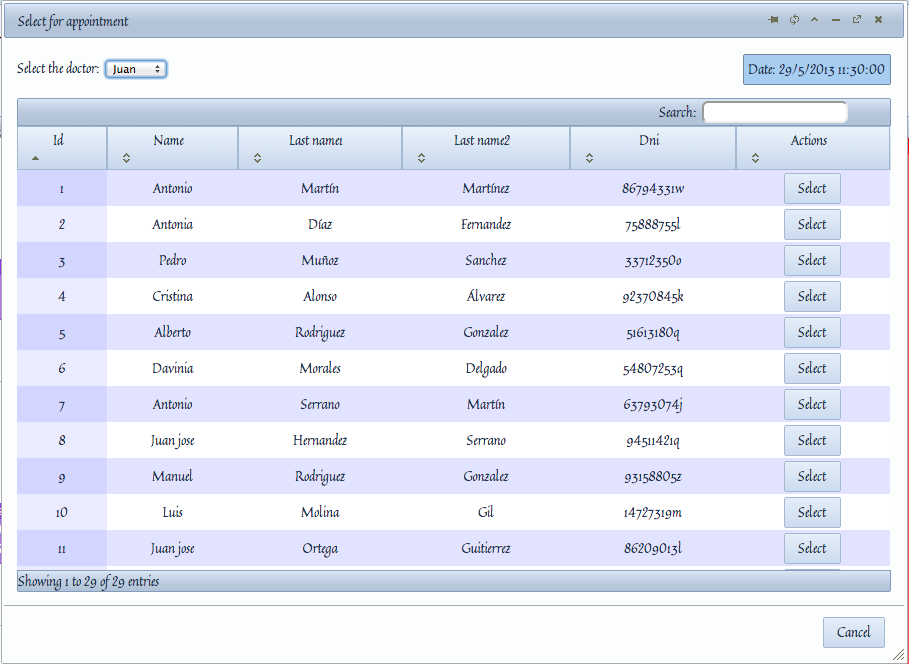
\includegraphics[scale=0.35]{icapcitas1.png}
  \caption{New appointment dialog screen}
  \label{a}
\end{figure}

In this screen, which appears when you click a cell in the calendar, you select the participants of the event. The doctor, who may be chosen in the top left, and only show the doctors that are available (discarding those with a permit on that date or the disabled). The customer can select in the table using the select button. If customer should choose a doctor or busy at that time the system would display an error, leaving the event store.

\newpage
\begin{figure}[!htb]
  \centering
    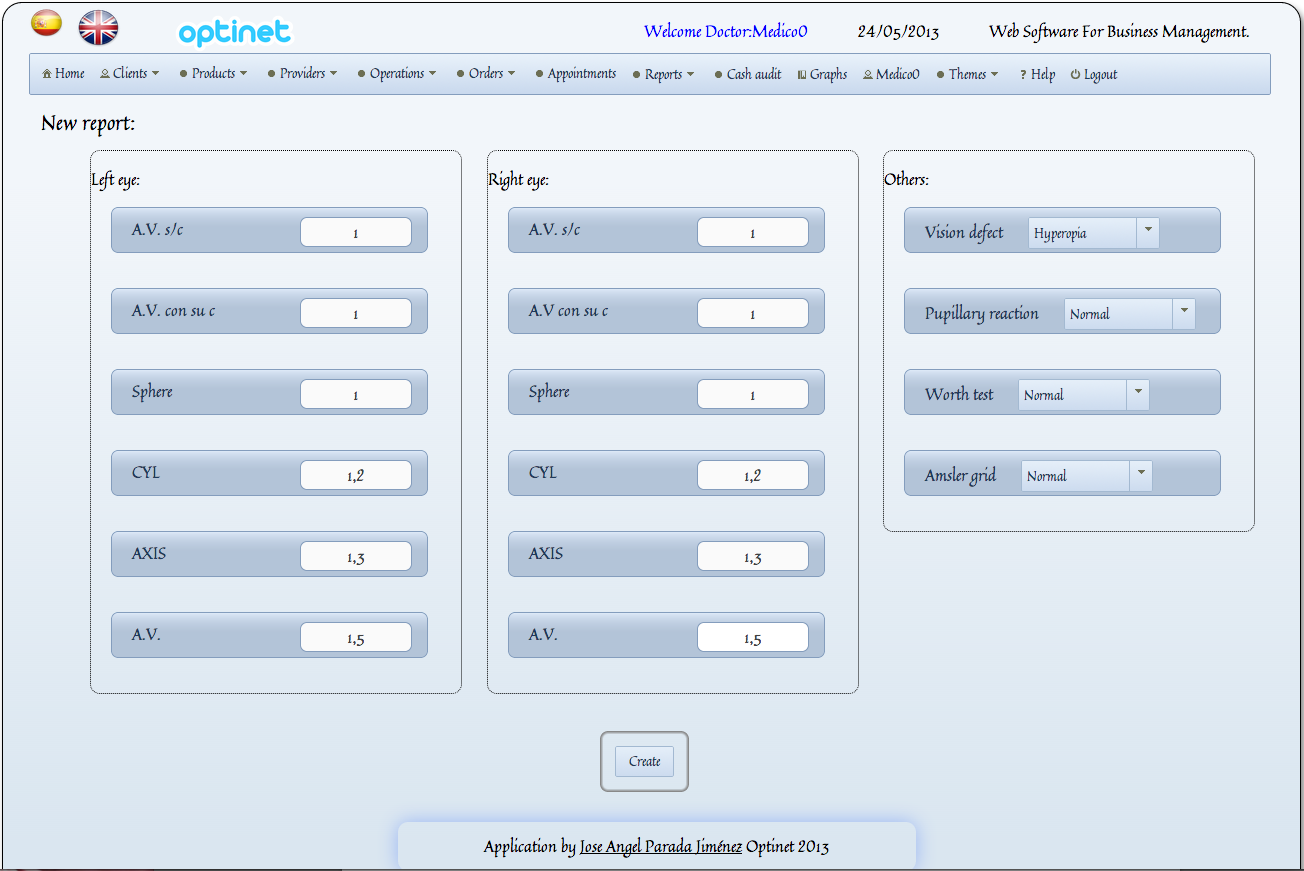
\includegraphics[scale=0.35]{icapregistrarinforme.png}
  \caption{Display new report}
  \label{a}
\end{figure}

The reports only doctors can perform and are not modifiable. The medical reports can be made in two different ways, by appointment or walk.\\If you chose the option without an appointment, it shows a table with customers stored in the system where the user select the one you want Give you the report. The system will store a date at the time of creating the report.\\If you chose the option with appointment calendar displays all appointments assigned to the physician that is connected to the doctor select the event you want to Give you the report.\\Appointments that have already made the report appear in the calendar are color black. Appointments that already have the report appear in the calendar made in black. If any appointment pulsase has already shown directly report the report.


\newpage
\subsection {Display record arching}

\begin{figure}[!htb]
  \centering
    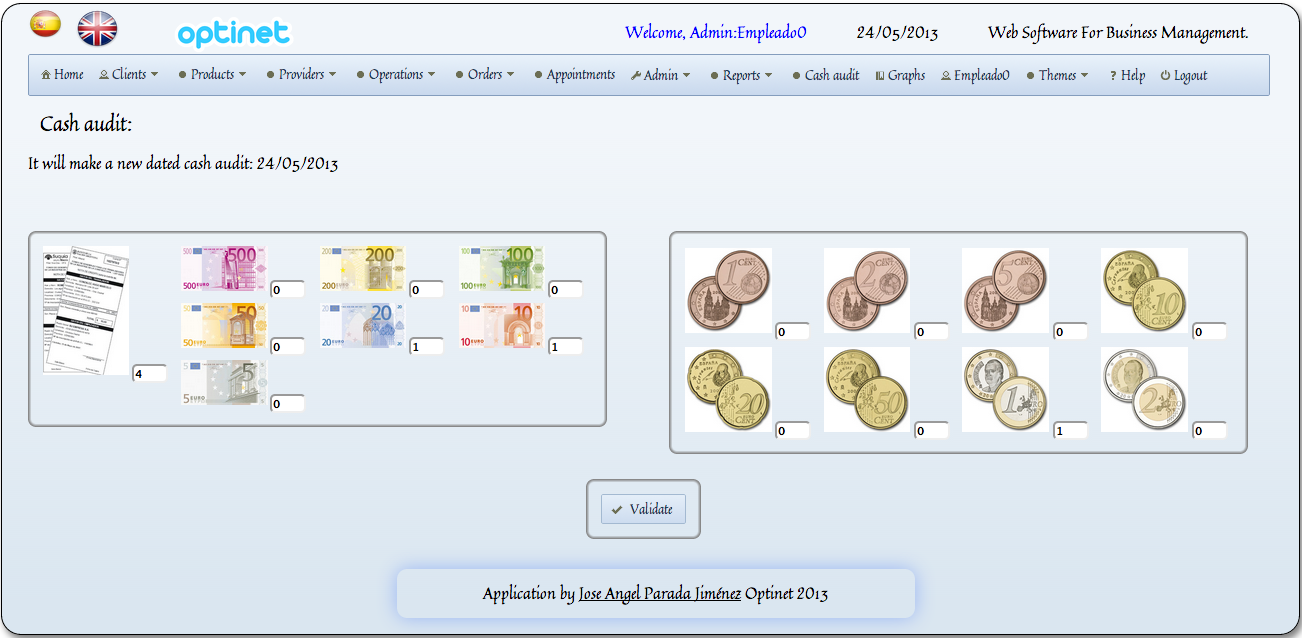
\includegraphics[scale=0.35]{icapnuevoarqueo.png}
  \caption{Display record arching}
  \label{a}
\end{figure}

In this screen the user can make the end of the day the count of the box. The system do not allow more than one daily arching showing a message and invalidating the button. The system displays an error message if it detects that there have been no data correctly. When the system makes checking the box, if it is correct arching is stored in the system but if instead the arching differs by more than 1 unit will display a arching NOT confirmed and offering the user the possibility of reintroducing data or otherwise save anyway.

\newpage
\subsection {Display user statistics}

\begin{figure}[!htb]
  \centering
    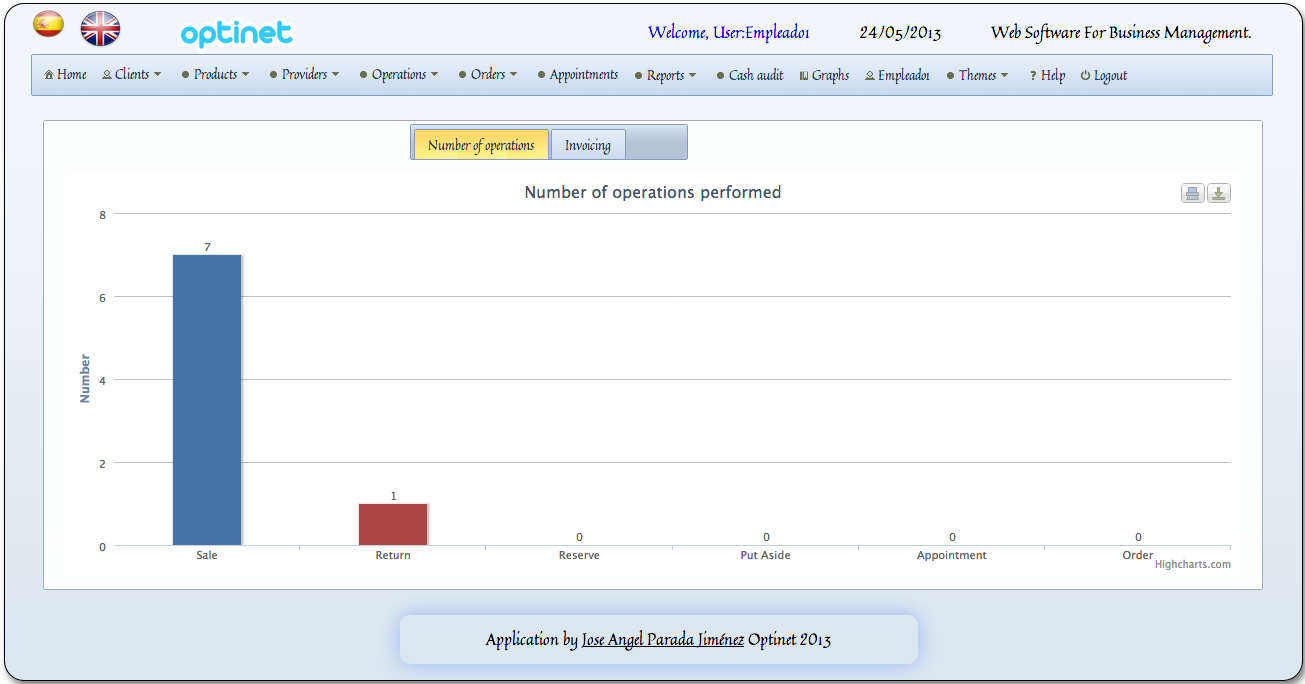
\includegraphics[scale=0.35]{icapestadisticasemp.png}
  \caption{Display user statistics}
  \label{a}
\end{figure}

In this screen the user can navigate through the menu to see their own statistics allows also the user to export the statistics to different formats and the ability to print. If the user pressed any bar graph show the list of operations associated with the graph.

\newpage
\subsection {Modify User Screen}

\begin{figure}[!htb]
  \centering
    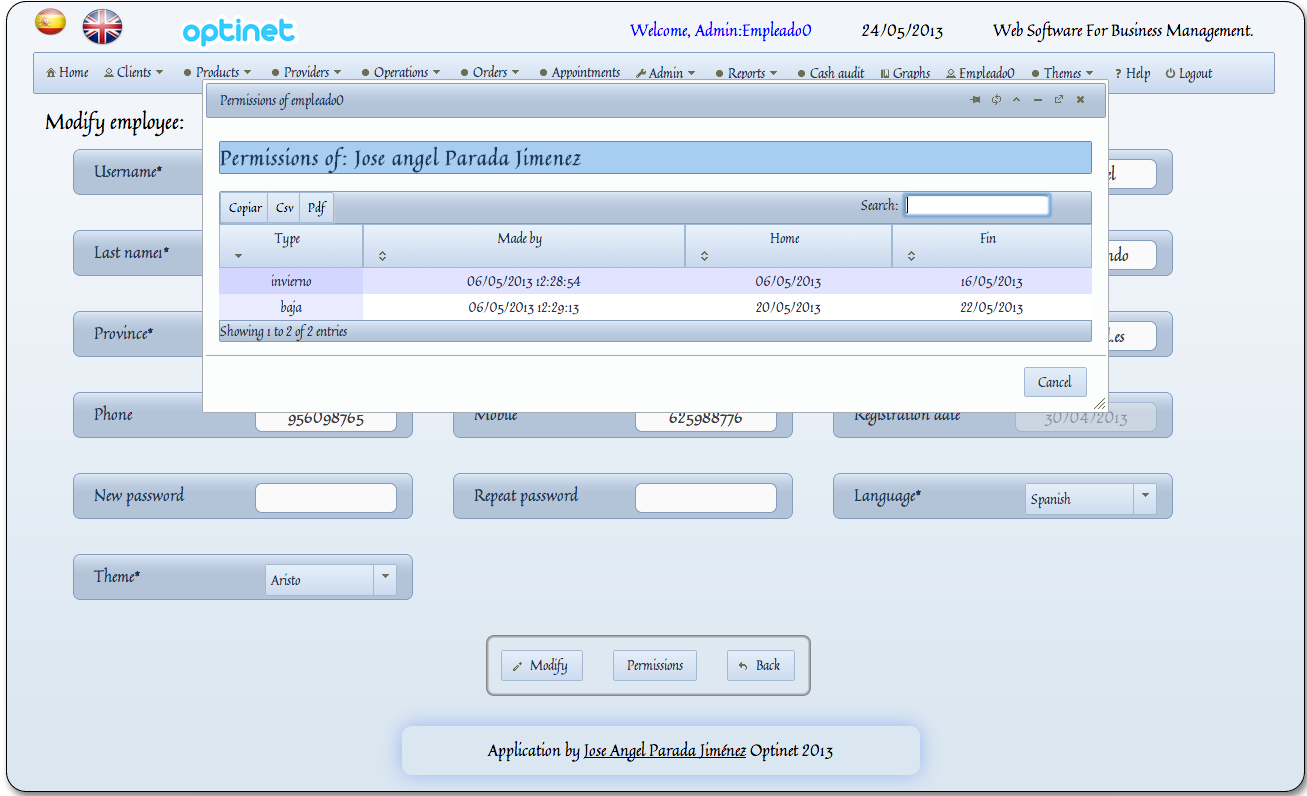
\includegraphics[scale=0.35]{icapmodificarempleado.png}
  \caption{Modify User Screen}
  \label{a}
\end{figure}

In this screen the user can modify the data and password. It also offers the ability to view or print the permissions assigned the administrator by clicking the Permissions button. If the user did not have any permission, the button will appear disabled.

\newpage
\subsection {Screen recording employee/doctor}

\begin{figure}[!htb]
  \centering
    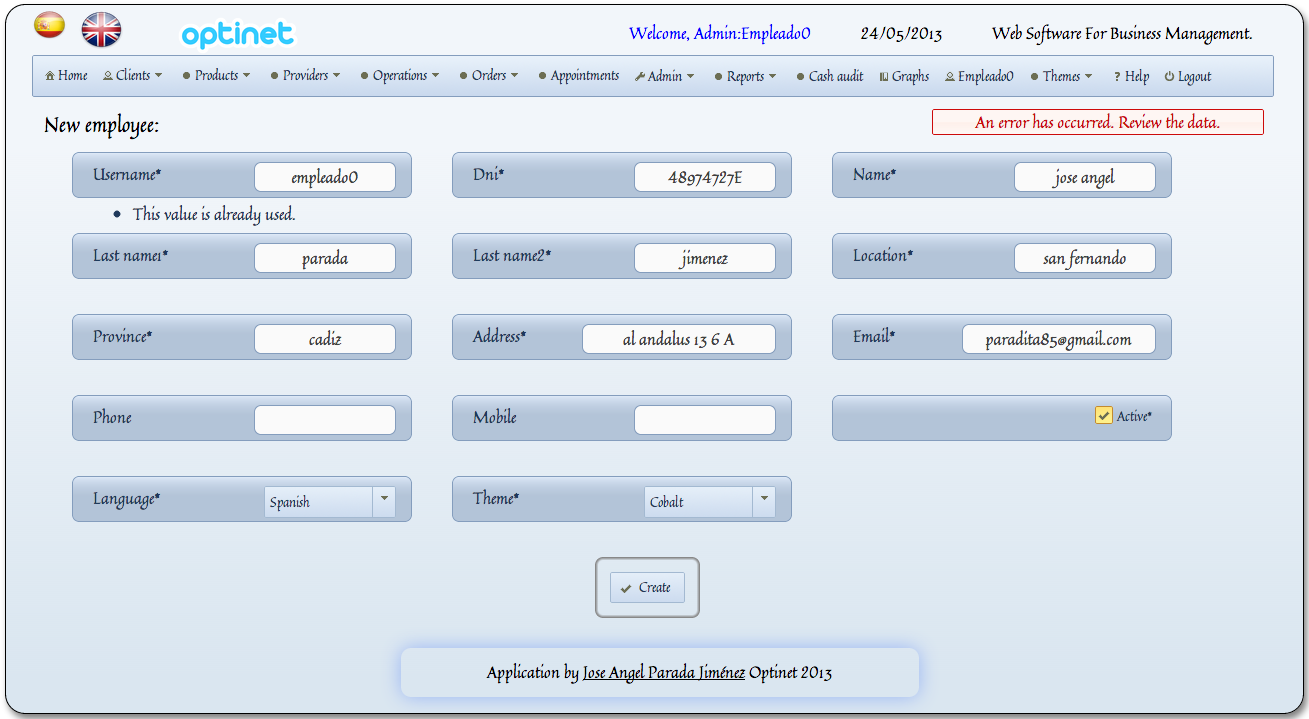
\includegraphics[scale=0.35]{icapregistroemp.png}
  \caption{Screen recording employee/doctor}
  \label{a}
\end{figure}

In this screen, the administrator can create a new user of the application. Not able to create two users with the same username or email and the system would fail. If the registration of a physician will be additional fields qualifications, number, color. The color needed to be painted and appointments for the doctor with the color chosen in the calendar of appointments.

\newpage
\subsection {Display list employees}

\begin{figure}[!htb]
  \centering
    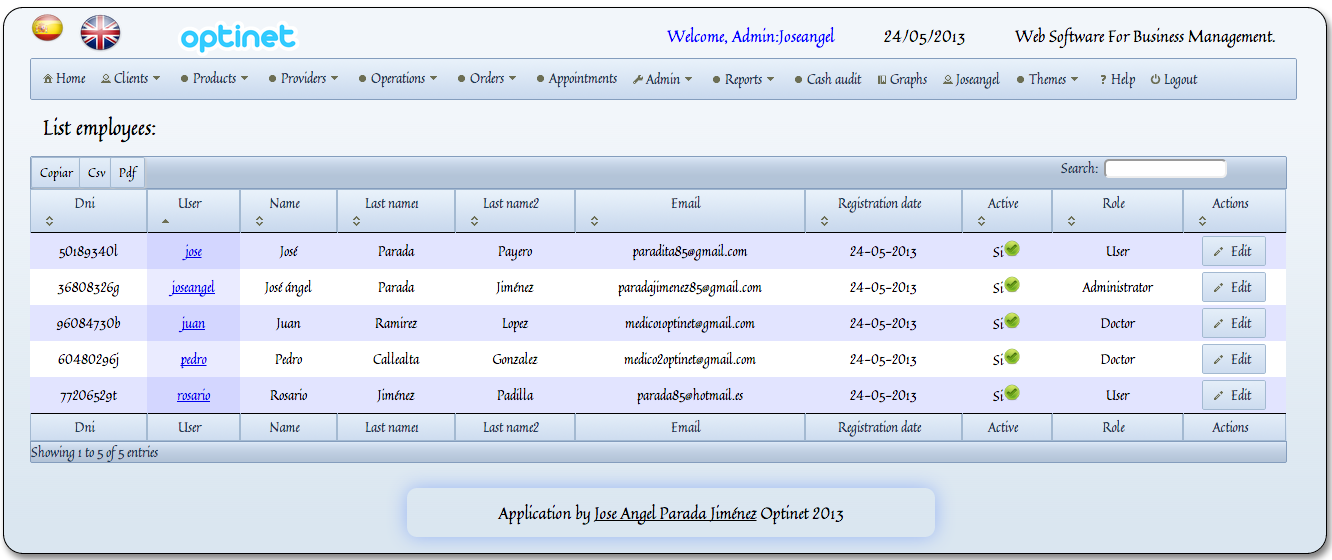
\includegraphics[scale=0.35]{icaplistarempleados.png}
  \caption{Display list employees}
  \label{a}
\end{figure}

On this screen, the administrator can view the application users. It offers the ability to edit any except application user password that only the user can know. The administrator only has the ability to send email back to the user a new password. The administrator is the only user of the application can not be disabled.

\newpage
\subsection {Display connections list}

\begin{figure}[!htb]
  \centering
    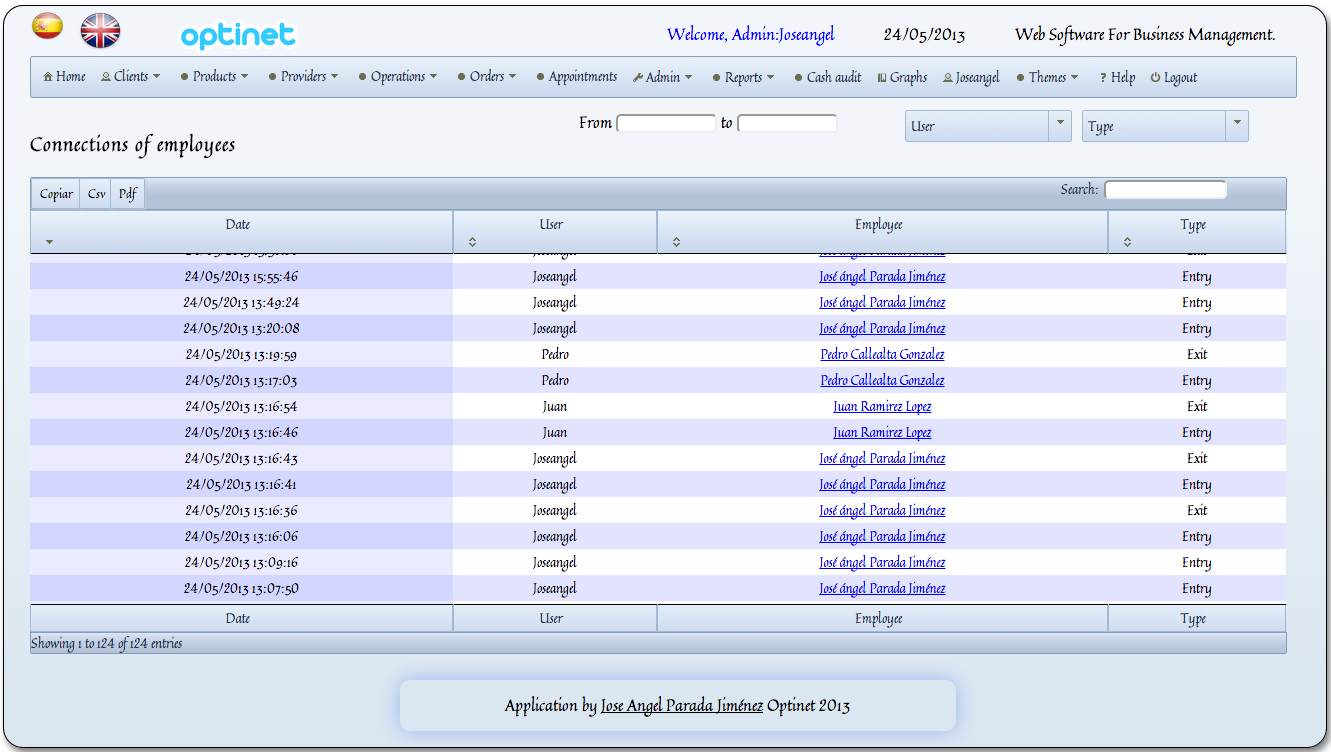
\includegraphics[scale=0.35]{icapconexiones.png}
  \caption{Display connections list}
  \label{a}
\end{figure}

On this screen, the administrator can check the connections to the system users. This allows you to have information when the system input and output of each employee.

\newpage
\subsection {List screen changes}

\begin{figure}[!htb]
  \centering
    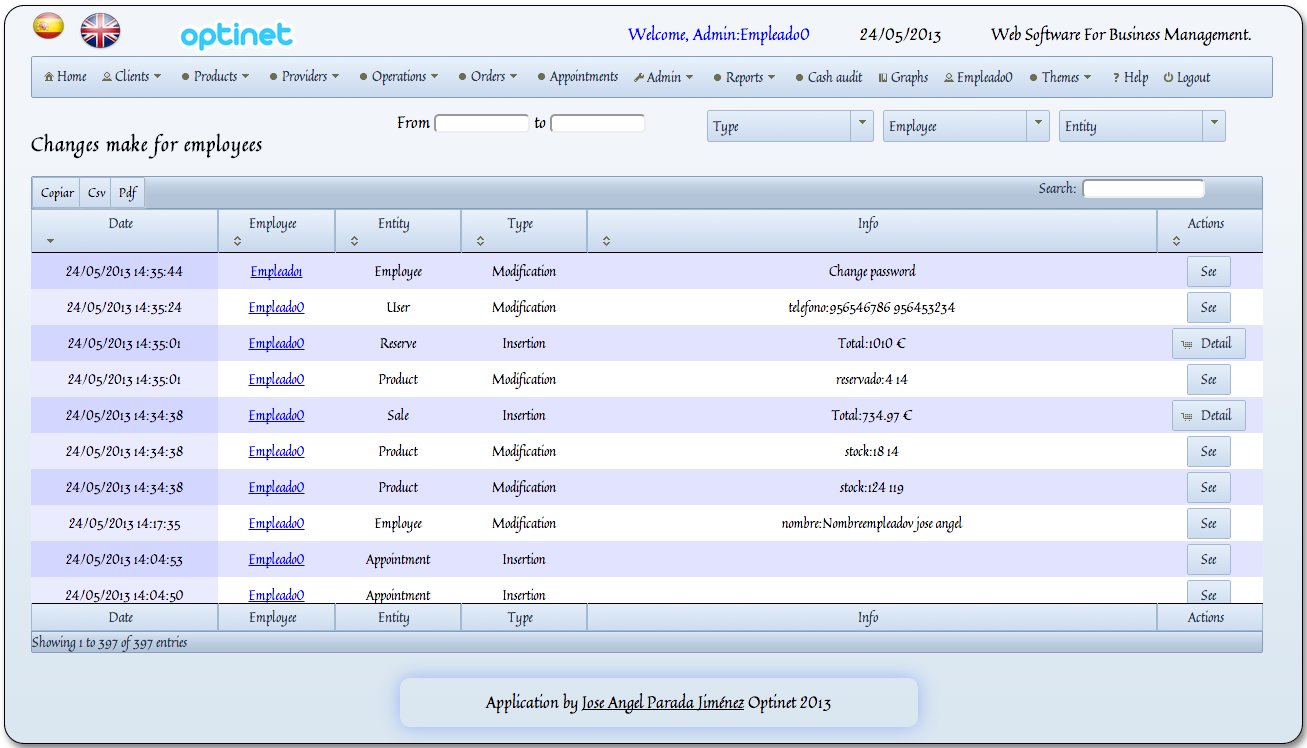
\includegraphics[scale=0.35]{icapcambios.png}
  \caption{List screen changes}
  \label{a}
\end{figure}

On this screen, the administrator can view the changes made to the system. If, for example, we changed the name to a client would be stored in the system the old name and who made the change, so the administrator will know at all times who has made some change in the system. If an administrator or an application user change his password, a message will changed password for the administrator can not see the password.

\newpage
\subsection {Display arching calendar}

\begin{figure}[!htb]
  \centering
    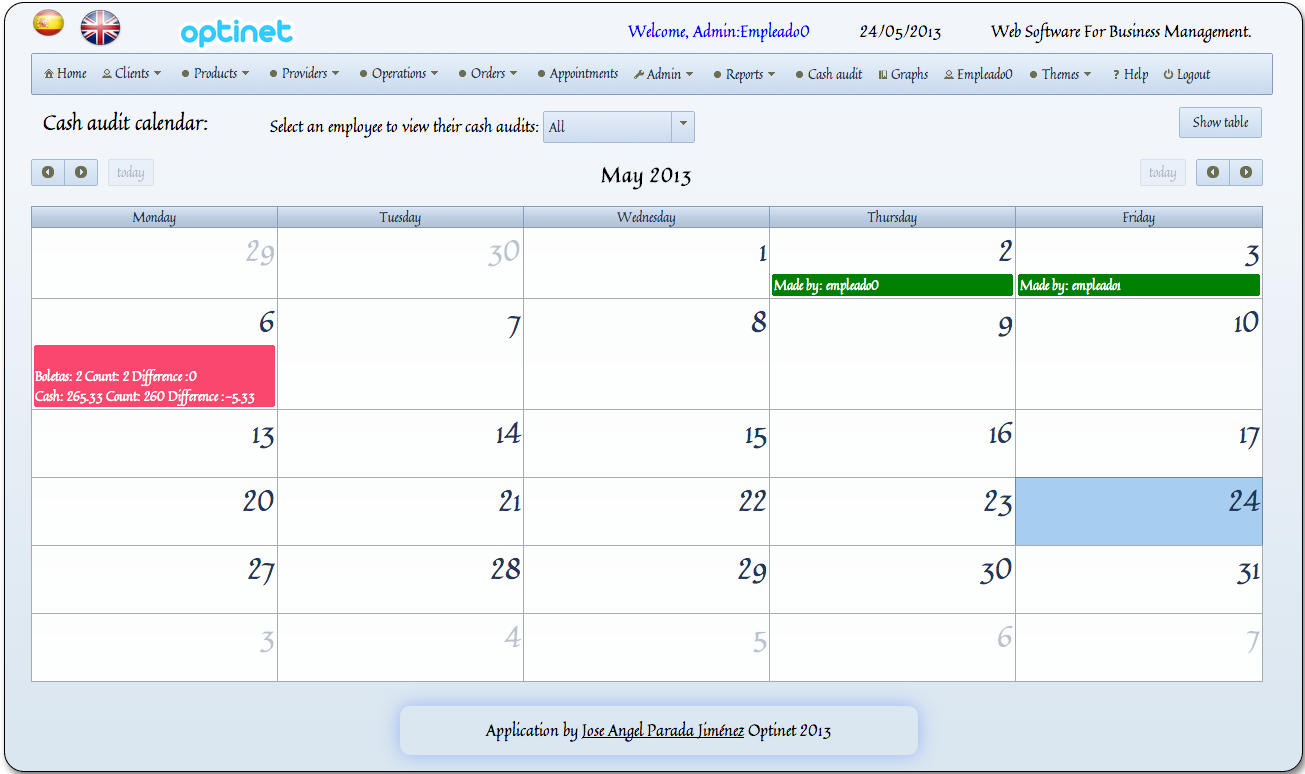
\includegraphics[scale=0.35]{icapcalendarioarqueos.png}
  \caption{Display arching calendar}
  \label{a}
\end{figure}

On this screen, the administrator can view the Arcing carried on the system. The Arcing confirmed schedule will be painted in green and red unconfirmed. If we let the pointer over any arching, will display the time and who performed the calibration. To search or simply print a list of Arcing can we turn to button the top right display table that displays all tonnages.


\newpage
\subsection {Display manage holidays}

\begin{figure}[!htb]
  \centering
    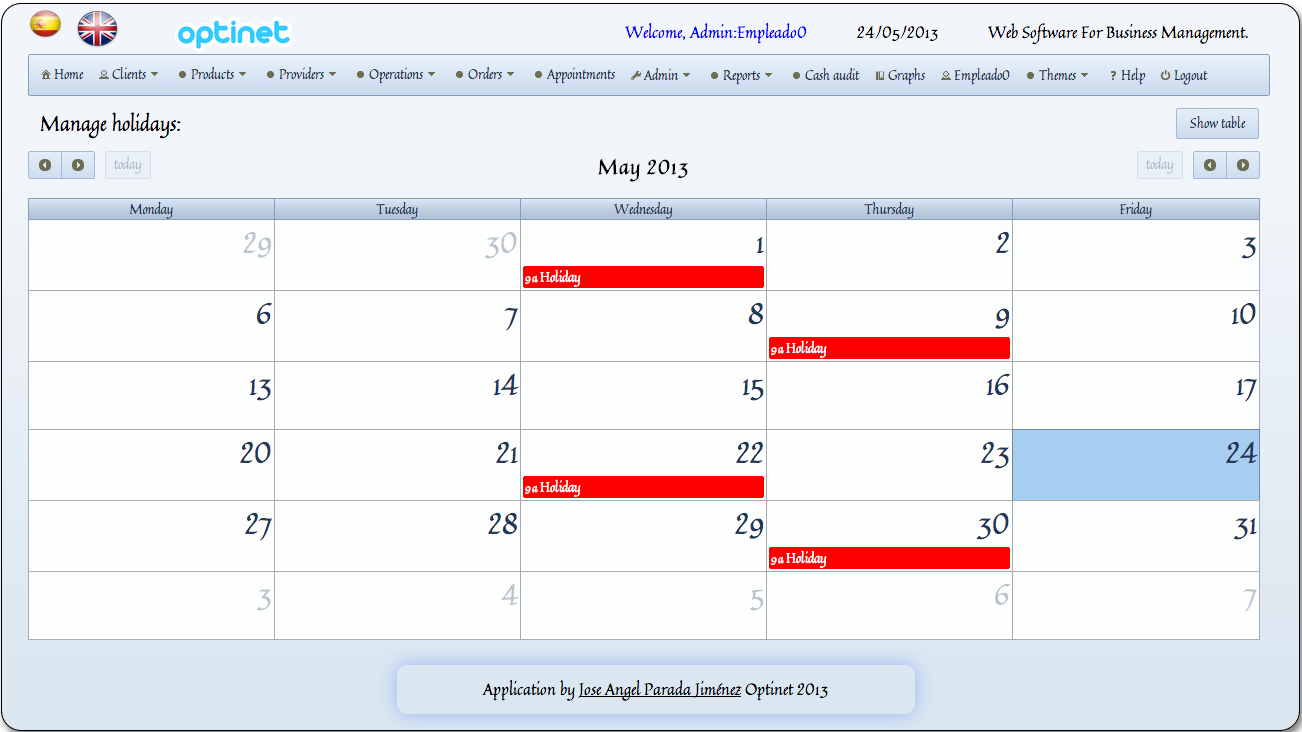
\includegraphics[scale=0.35]{icapfestivos.png}
  \caption{Display manage holidays}
  \label{a}
\end{figure}

On this screen, the administrator can manage the holidays. To create a new festive be pressed on the chosen day. To delete a festive holiday pressed in to be deleted. You may not create a holiday on a day where there already citas.Existe the ability to display a table of stored holidays clicking the top right button show table.

\newpage
\subsection {Display manage permissions}

\begin{figure}[!htb]
  \centering
    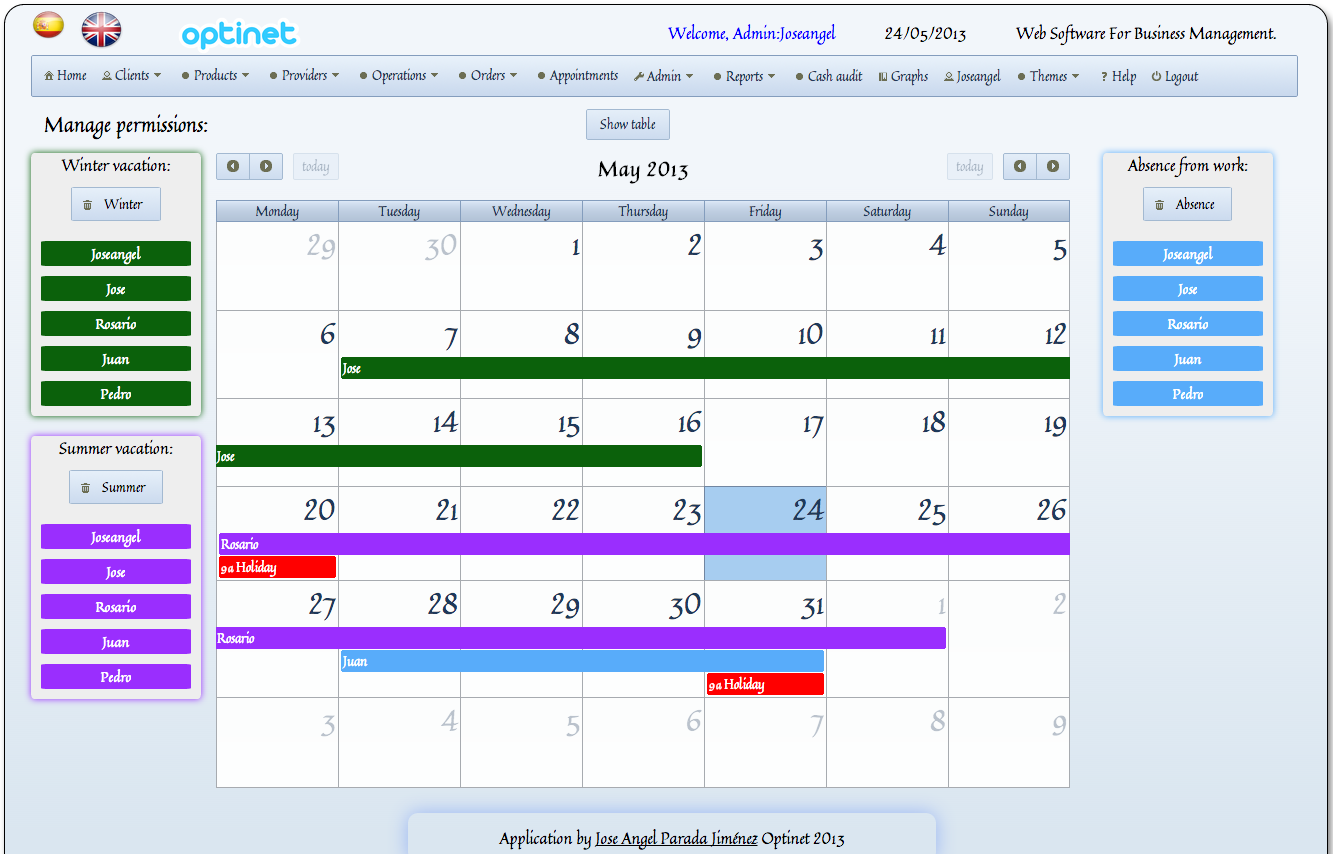
\includegraphics[scale=0.35]{icappermisos.png}
  \caption{Display manage permissions}
  \label{a}
\end{figure}

In this screen, the administrator can manage the permissions associated with users of the system. Permissions are assigned to calendar dragging the chosen day. Permissions can be lengthened or shortened everything you want. Permits may be removed by clicking on them, or if you would like to delete all permissions for a particular type would press its button. It is possible to display the permissions on a table in order to print or simply search permits faster. There are some restrictions:
\begin{itemize}
\item Can not create a vacation in the same year. Eg winter holiday twice in the same year.
\item Not a single employee can have more than one license for the same date. Eg a sick leave and summer vacation.
\end{itemize}

\newpage
\subsection {Display statistics}

\begin{figure}[!htb]
  \centering
    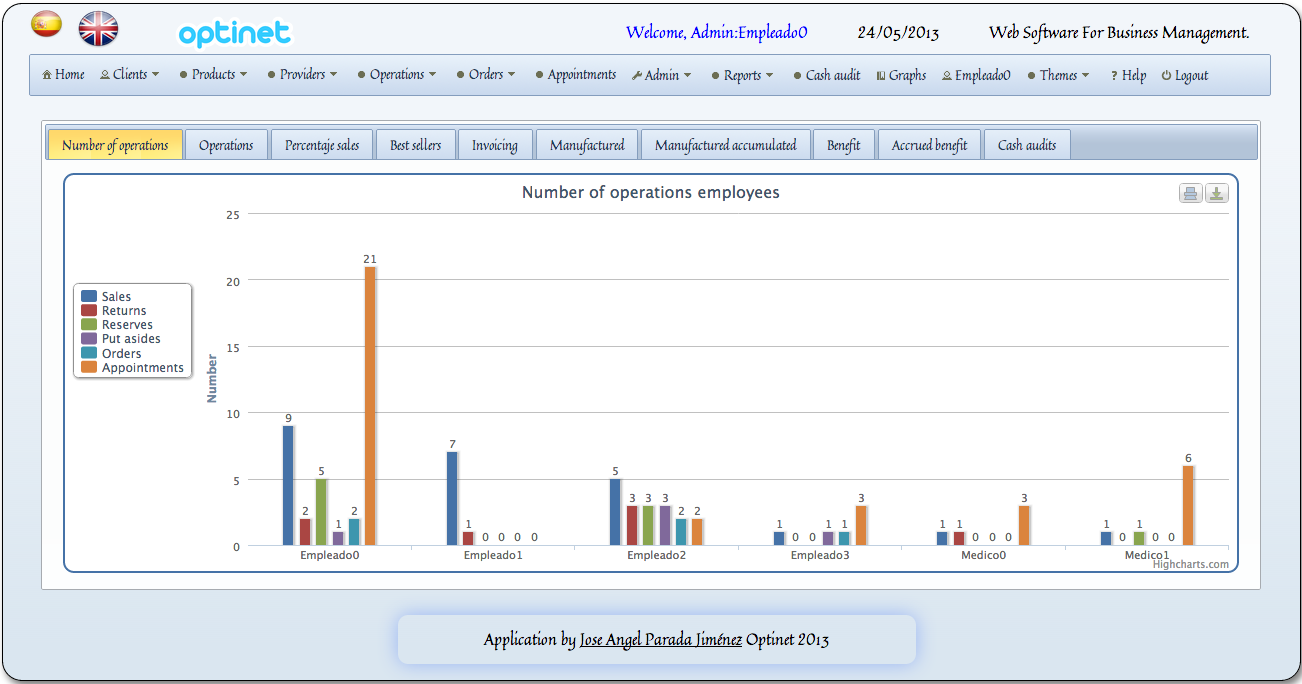
\includegraphics[scale=0.35]{icapestadisticas.png}
  \caption{Display statistics}
  \label{a}
\end{figure}

\begin{figure}[!htb]
  \centering
    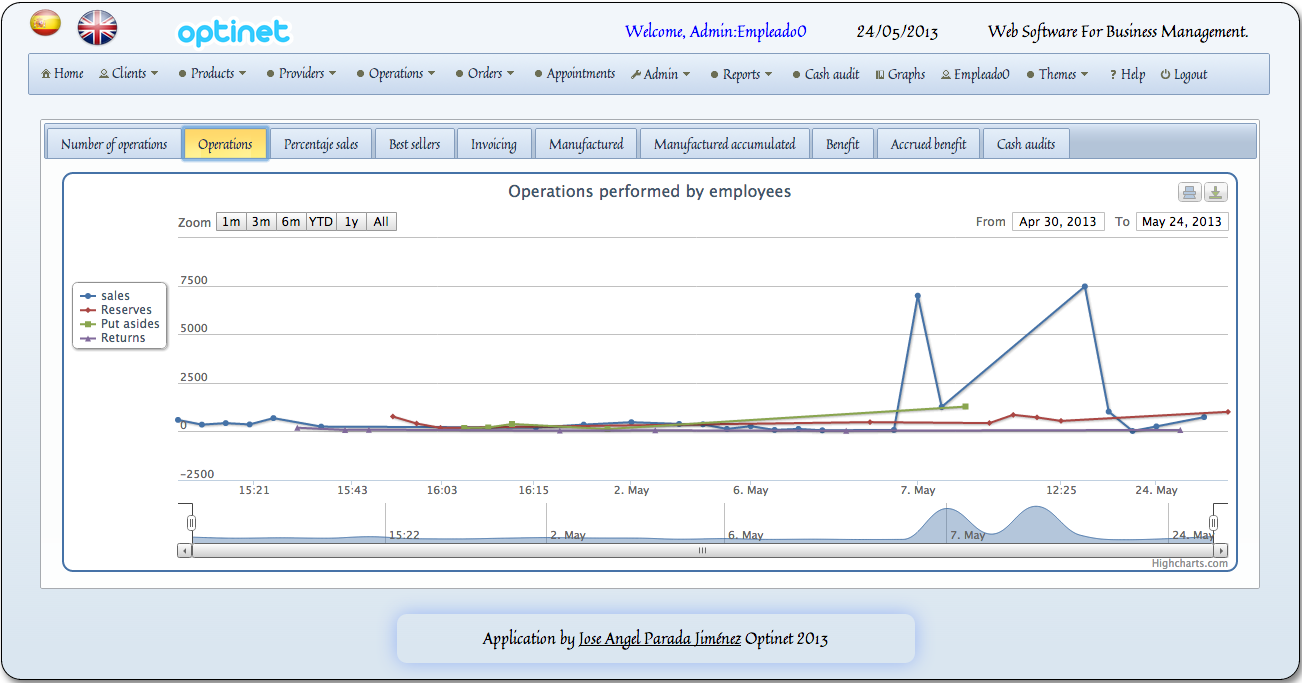
\includegraphics[scale=0.35]{icapestadisticas1.png}
  \caption{Display statistics 1}
  \label{a}
\end{figure}

\newpage
\begin{figure}[!htb]
  \centering
    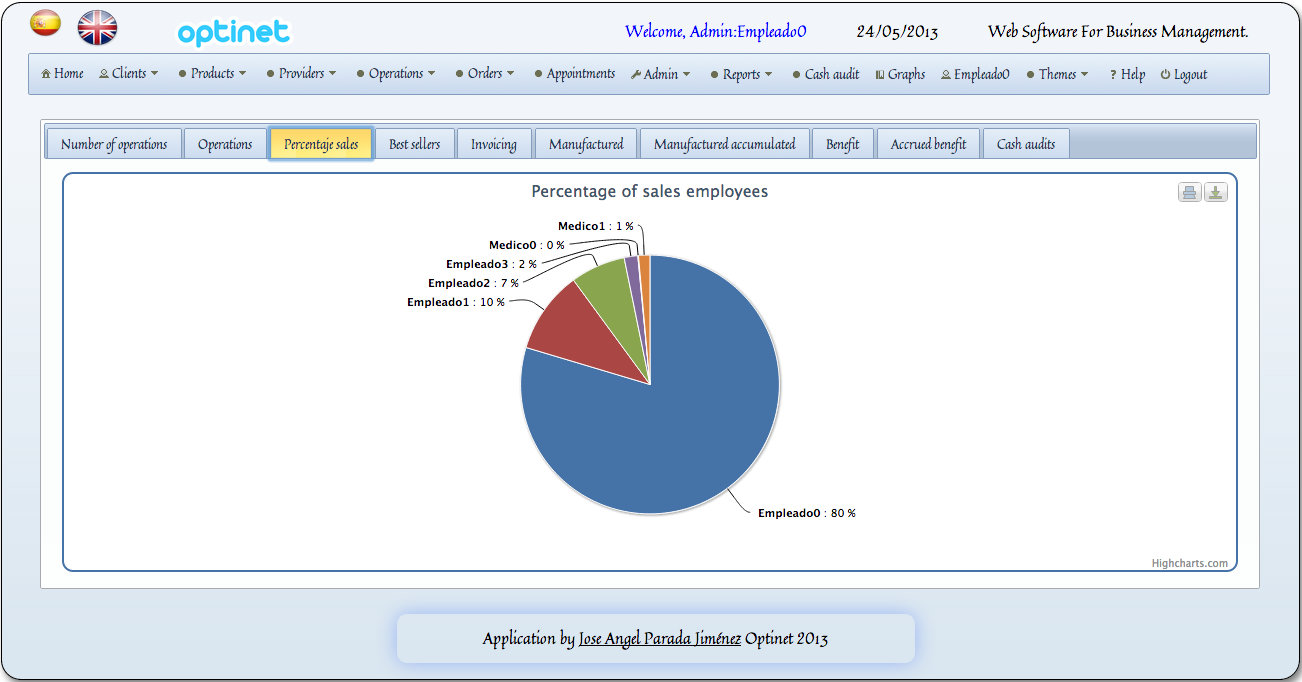
\includegraphics[scale=0.35]{icapestadisticas2.png}
  \caption{Display statistics 2}
  \label{a}
\end{figure}

\begin{figure}[!htb]
  \centering
    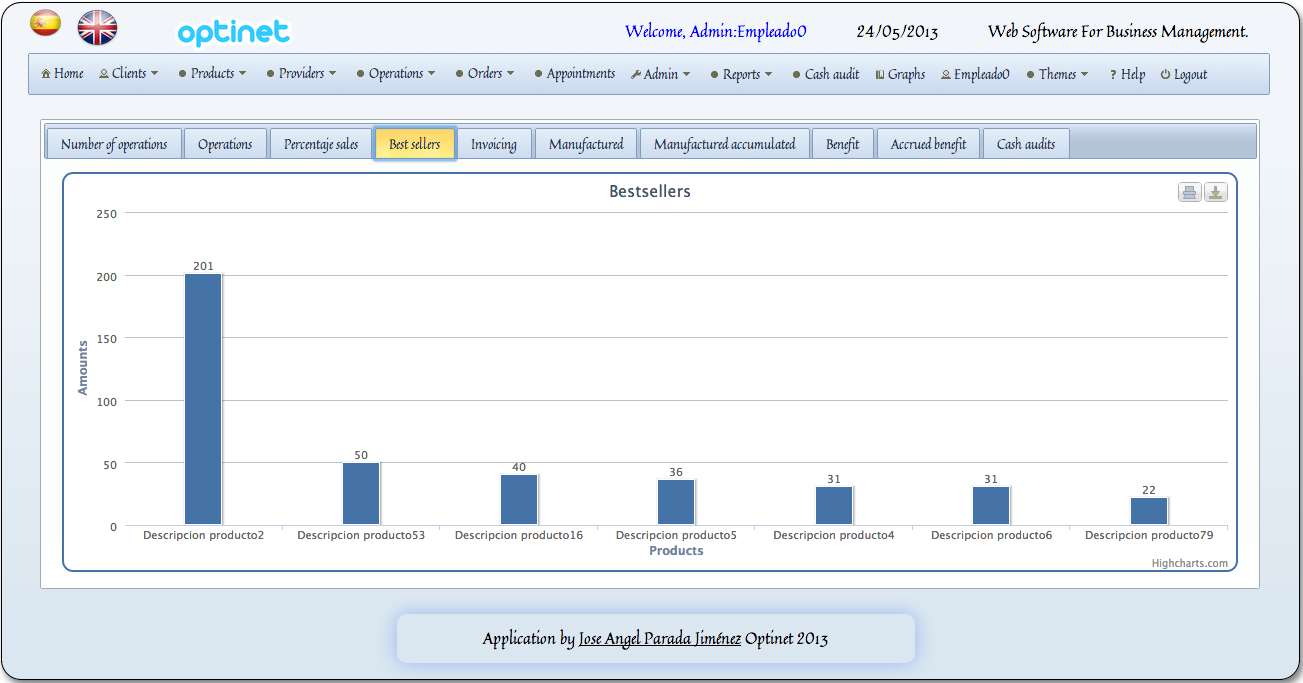
\includegraphics[scale=0.35]{icapestadisticas3.png}
  \caption{Display statistics 3}
  \label{a}
\end{figure}
On this screen, the administrator can view all system information graphically. All generated graphs offering print or store by clicking the icons at the top right. In the center of the top of the graph shows the description of each graph.

\end{document}
